\documentclass{beamer}
%\documentclass[handout]{beamer}

% \usepackage{ensislidesOG}
%\usepackage[utf8]{inputenc}
% \usepackage[T1]{fontenc}
\usepackage[english]{babel}
\usepackage[sfdefault]{roboto} 
\usepackage{amsfonts}
\usepackage{amsmath}
\usepackage{amssymb}
\usepackage{amsthm}
% \usepackage[frenchstyle]{mathalpha}
% \usepackage[OMLmathsfit]{isomath}
\usepackage{graphicx}
\usepackage{color} % for ps_tex inclusions
\usepackage{fmtcount} % th, e.g. \ordinalnum{4}
\usepackage{booktabs}
\usepackage{xr}
\usepackage{hyperref}
\externaldocument[notes-]{notes}

\newcommand{\itb}{\item[$\bullet$]}
\newcommand{\dps}{\displaystyle}

\usetheme{Madrid}
\usecolortheme{seagull}


\def\<{{\guillemotleft}}
\def\>{{\guillemotright}}

\def\vs1{\vspace{1mm}}
\def\v3{\vspace{3mm}}

\newcommand{\II}{\,\mbox{I\hskip -0.600em 1}}

\newcommand{\ME}{{\mathcal E}}
\newcommand{\MN}{{\mathcal N}}

\newcommand{\NN}{\ensuremath{\mathbb{N}}}
\newcommand{\RR}{\ensuremath{\mathbb{R}}}

\newcommand{\card}{\mbox{card}}
\newcommand{\pa}{\mbox{pa}}

\newcommand{\De}{\mbox{De}}
\newcommand{\Nd}{\mbox{Nd}}
\newcommand{\Ne}{\mbox{Ne}}

\newcommand{\indep}{\perp\!\!\!\perp}
\newcommand{\condindep}[3]{#1 \indep #2 \vert #3}
\newcommand{\condindepP}[4]{#1 \indep_{#4} #2 \vert #3}
\newcommand{\ts}[3]{#1_{#2}^{#3}}
\newcommand{\set}[1]{\{#1\}}

\newcommand{\bs}[1]{\boldsymbol{#1}}


\definecolor{mypurple}{RGB}{200,0,255}


\title[LPC]{Learning, Probabilities and Causality}

\subtitle{Chapter I - Introduction and Conditional Independence}

\author[Xavi and Thomas]{Xavier Alameda-Pineda and Thomas Hueber}

\institute{Ensimag/Inria/CNRS/Univ. Grenoble-Alpes}

\makeatother
\setbeamertemplate{footline}
{
  \leavevmode%
%   \hbox{%
%   \begin{beamercolorbox}[wd=.4\paperwidth,ht=2.25ex,dp=1ex,center]{author in head/foot}%
%     \usebeamerfont{author in head/foot}\insertshortauthor
%   \end{beamercolorbox}%
%   \begin{beamercolorbox}[wd=.6\paperwidth,ht=2.25ex,dp=1ex,center]{title in head/foot}%
    \usebeamerfont{title in head/foot}\hfill
    \insertframenumber{} / \inserttotalframenumber\hspace*{1ex}
%   \end{beamercolorbox}}%
%   \vskip0pt%
}
\makeatletter
\setbeamertemplate{navigation symbols}{}

\AtBeginSection[]{
  \begin{frame}
  \vfill
  \centering
  \begin{beamercolorbox}[sep=8pt,center,shadow=true,rounded=true]{title}
    \usebeamerfont{title}\insertsectionhead\par%
  \end{beamercolorbox}
  \vfill
  \end{frame}
}

\AtBeginSubsection[]{
  \begin{frame}
  \vfill
  \centering
  \begin{beamercolorbox}[sep=8pt,center,shadow=true,rounded=true]{title}
    \usebeamerfont{title}\insertsectionhead\\---\\\insertsubsectionhead\par%
  \end{beamercolorbox}
  \vfill
  \end{frame}
}

\date{}

\newcommand{\exercise}[2]{\noindent\colorbox{blue!10}{\parbox{0.995\textwidth}{\textbf{Exercise \ref{notes-ex:#1}}: #2}}\\}
\newcommand{\remark}[2]{\noindent\colorbox{red!10}{\parbox{0.995\textwidth}{\textbf{Remark \ref{notes-rmk:#1}}: #2}}\\}

%%%%%%%%%%%%%%%%%%%%%%%%%%%%%%%%%%%%%%%%%%%%%%%%%%%%%%%%%%%%%%

\begin{document}

\begin{frame}
  \titlepage
\end{frame}

\begin{frame}{Table of Today's Contents}
 \tableofcontents
\end{frame}

%%%%%%%%%%%%%%%%%%%%%%%%%%%%%%%%%%%%%%%%%%%%%%%%%%%%%%%%%%%%%%
\section[Course Organisation]{Course Organisation}
%%%%%%%%%%%%%%%%%%%%%%%%%%%%%%%%%%%%%%%%%%%%%%%%%%%%%%%%%%%%%%

%%%%%%%%%%%%%%%%%%%%%%%%%%%%%%%%%%%%%%%%%%%%%%%%%%%%%%%%%%%%%%
\begin{frame}{Course Content}
Learning Probabilities and Causality is structured in two parts.
 \begin{enumerate}
  \item Learning for probabilistic models given a causality graph\\ (Thomas \& Xavi)
  \item Methods for inferring this graph from data\\ (Emilie \& Eric)
 \end{enumerate}
 \begin{figure}[H]
  \centering
  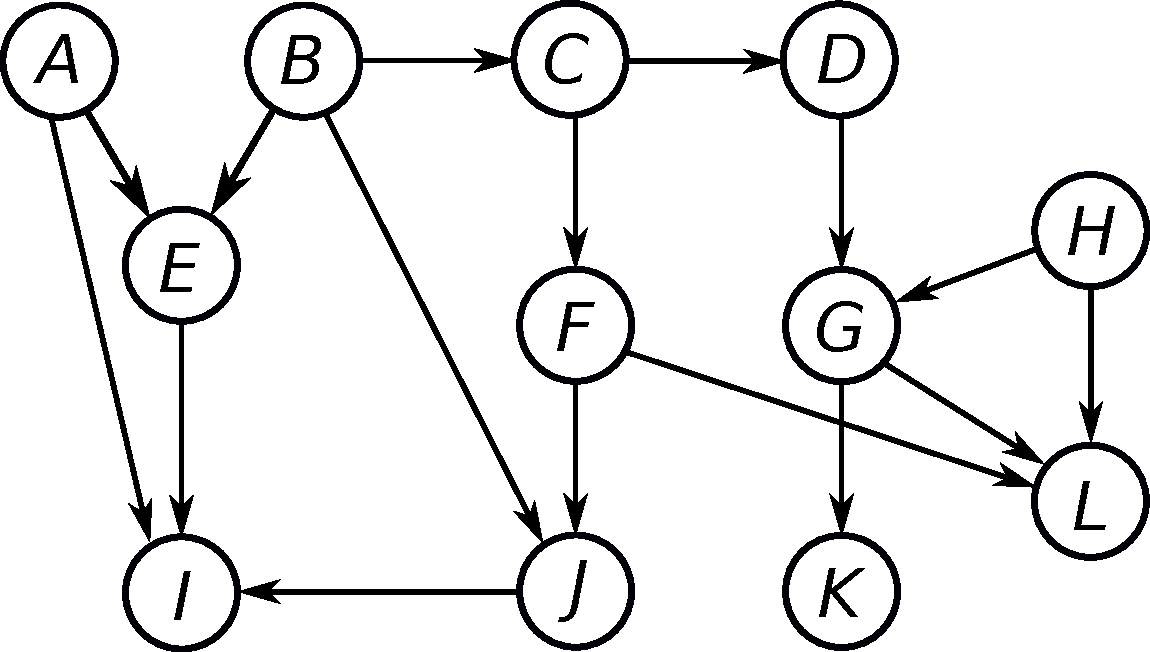
\includegraphics[width=0.4\textwidth]{fig/D-separation.pdf}
 \end{figure}

\end{frame}


%%%%%%%%%%%%%%%%%%%%%%%%%%%%%%%%%%%%%%%%%%%%%%%%%%%%%%%%%%%%%%
\begin{frame}{Course Content - Part 1}
Probabilistic learning with latent variables:\vspace{5mm}
 \begin{enumerate}
  \item Basics of probabilistic models: {\bf conditional independence}
  \item Model-based clustering and {\bf Gaussian} mixture models
  \item Sequential data and hidden {\bf Markov} models
  \item Probabilistic principal component analysis
  \item Linear dynamical systems
  \item Approximate variational inference
 \end{enumerate}
%  \pause
%  \begin{block}{Changes} 
% We added variational inference and reduced the length fo the first chapter. Variational methods (i.e.\ VAE) are more and more popular, and it is important you know about the basics.  
%  \end{block}

\end{frame}


\begin{frame}{LPC Part 1 - Instructors}
 \begin{columns}
  \begin{column}{0.25\textwidth}
  
\includegraphics[width=\textwidth]{fig/hueber.jpg} 
  \end{column}
  \begin{column}{0.7\textwidth}
   Research Scientist [\alert{\href{http://www.gipsa-lab.fr/~thomas.hueber}{website}}] @thomashueber\\
   \texttt{thomas.hueber@gipsa-lab.fr}\\
    Leader of CRISSP (cognitive robotics, interactive systems, speech processing), GIPSA-Lab, CNRS\vspace{5mm}\\
    Multimodal speech processing, machine learning, interactive systems
  \end{column}
 \end{columns}\vspace{5mm}
%  \hrule\vspace{2mm}
 \begin{columns}
  \begin{column}{0.25\textwidth}
  \includegraphics[width=\textwidth]{fig/xavi-square.jpg} 
  \end{column}
  \begin{column}{0.7\textwidth}
   Research Scientist [\href{http://xavirema.eu}{\alert{webpage}}] @xavirema\\
   \texttt{xavier.alameda-pineda@inria.fr}\\
   Perception Team, Inria Grenoble Rh\^one-Alpes\vspace{5mm}\\
   Audio-visual perception, probabilistic and deep learning, human-robot interaction
  \end{column}
 \end{columns}
\end{frame}

%%%%%%%%%%%%%%%%%%%%%%%%%%%%%%%%%%%%%%%%%%%%%%%%%%%%%%%%%%%%%%
\begin{frame} \frametitle{Grading Rules}
	\begin{itemize}
		\item Lab work (LW), mid-term exam (ME) final exam (FE).
		\item Grade = (LW+ME+FE)/3.
		\item LW = average of all lab works.
	\end{itemize}
	\vspace{3mm}
	{\bf Support material}: \texttt{https://chamilo.grenoble-inp.fr/courses/ENSIMAGWMM9AM46}.
\end{frame}

\begin{frame}{Calendar}
\centering 
 \begin{tabular}{rccc}
  \toprule
  When? & Who? & Where? & Comment\\
  \midrule
  30-Sep & Xavi & D211 \\
  7-Oct & Thomas & D207 \\
  14-Oct & Thomas & D207 \& E303 & Lab (15h30-17h)\\
  21-Oct & Xavi & D111 \\
  28-Oct & Xavi & H105 \\
  18-Nov & Xavi & D111/E303 & Lab (15h30-17h)\\
  25-Nov & Emilie/Eric & H105 & Mid-term Exam (14h-15h30) \\
  2-Dec & Emilie/Charles & H105\\
  9-Dec & Emilie & E201 & Lab (14h-17h)\\
  16-Dec & Eric/Charles & H105\\
  6-Jan & Charles/Emilie & H105 \\
  13 Jan & Charles/Eric & H105/E200 & Lab (15h30-17h)\\
  \bottomrule
 \end{tabular}
\end{frame}


%%%%%%%%%%%%%%%%%%%%%%%%%%%%%%%%%%%%%%%%%%%%%%%%%%%%%%%%%%%%%%
\begin{frame} \frametitle{References}
There is \textbf{a lot} of bibliography on probabilistic graphical models.\vspace{0.3cm}

I strongly suggest the following book:\vspace{0.4cm}\\

\begin{columns}
  \begin{column}{0.3\textwidth}%
   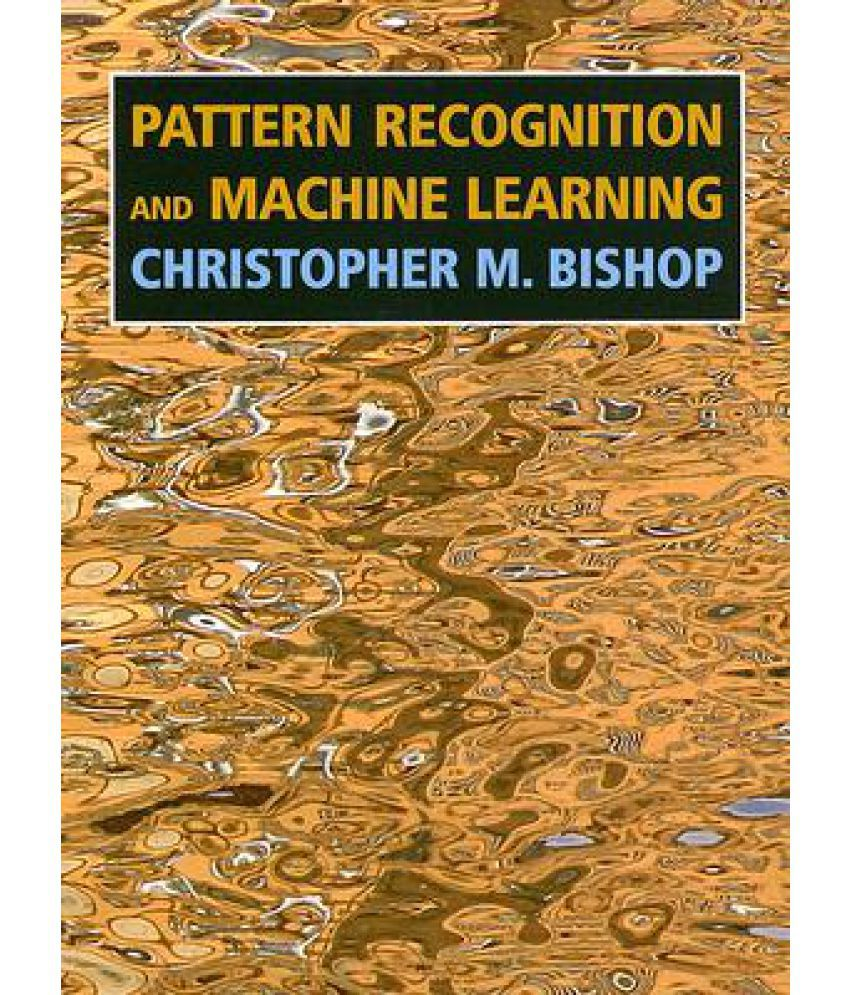
\includegraphics[width=\textwidth]{fig/bishopbook.jpg}
  \end{column}%
  \begin{column}{0.6\textwidth}
    \textit{Pattern Recognition and Machine Learning}, from Christopher M. Bishop (Springer)\vspace{0.4cm}\\
    The concepts discussed in FPDM correspond to different parts of Ch. 2, 8, 9, 10, 12, 13.\vspace{0.4cm}\\
    You will not find the part on variational autoencoders (last chapter).
  \end{column}
 \end{columns} 
\end{frame}

% %%%%%%%%%%%%%%%%%%%%%%%%%%%%%%%%%%%%%%%%%%%%%%%%%%%%%%%%%%%%%%
% \begin{frame} \frametitle{Resources}
% \alert{
%     \begin{itemize}
%         \item The slides of the courses, future data sets and scripts are on 
%         {\url{http://chamilo.grenoble-inp.fr/courses/ENSIMAGWMM9AM21/}}
%         \item Also contains reminders on the pre-requisites, and some booklet (same contents as slides).
% 	\end{itemize}
% 	}
% \end{frame}

%%%%%%%%%%%%%%%%%%%%%%%%%%%%%%%%%%%%%%%%%%%%%%%%%%%%%%%%%%%%%%
\section{Introduction and Motivation}
%%%%%%%%%%%%%%%%%%%%%%%%%%%%%%%%%%%%%%%%%%%%%%%%%%%%%%%%%%%%%%

%%%%%%%%%%%%%%%%%%%%%%%%%%%%%%%%%%%%%%%%%%%%%%%%%%%%%%%%%%%%%%
\begin{frame} \frametitle{What is probabilistic data mining?}
\begin{itemize}
\item Probabilistic means we {\bf model} our data  using probabilities.
\item For example in classification, we aim to estimate the posterior probability: $P(c|x)$ for every possible class $c$.
\item Probabilistic generative models \& Bayes rule:
\[p(x,c) = p(x|c)p(c) \quad\Rightarrow\quad p(c|x) = \frac{p(x|c)p(c)}{\sum\limits_k p(x|k)p(k)} \]
\item What are all these ``$p$''? What do they mean?
\end{itemize}
\end{frame}

%%%%%%%%%%%%%%%%%%%%%%%%%%%%%%%%%%%%%%%%%%%%%%%%%%%%%%%%%%%%%%
\begin{frame}{Probabilities}
For {\bf discrete variables} (i.e.\ measurable events are discrete):
\[ p(c) = P(C=c). \]
$\rightarrow$ the probability of the random variable $C$ to value event $c$.\vspace{7mm}\\
For {\bf continuous variables} (i.e.\ measurable events are continuous):
\[ p(x) = f_X(x) \quad \text{and} \quad p({\cal X})=P(x\in{\cal X})=\int_{\cal X}f_X(x)\textrm{d}x \]
$f_X$ is the probability density function. Remember $P(\{x\})=0$.
\end{frame}

%%%%%%%%%%%%%%%%%%%%%%%%%%%%%%%%%%%%%%%%%%%%%%%%%%%%%%%%%%%%%%
\begin{frame} \frametitle{Why probabilistic data mining?}
\begin{itemize}
\item Infer hidden variables / exploit partly missing data
\item Example: clustering, image segmentation
\item Incorporate particular requirements in clustering
\item Model complex data (on grids, graphs, temporal, ...)
\item Simulate phenomena (speech synthesis), 
make predictions (regime switching in time series)
\end{itemize}
\begin{center}
	\begin{columns}
		\begin{column}{0.1\textwidth}
		\end{column}
		\begin{column}{0.5\textwidth}
			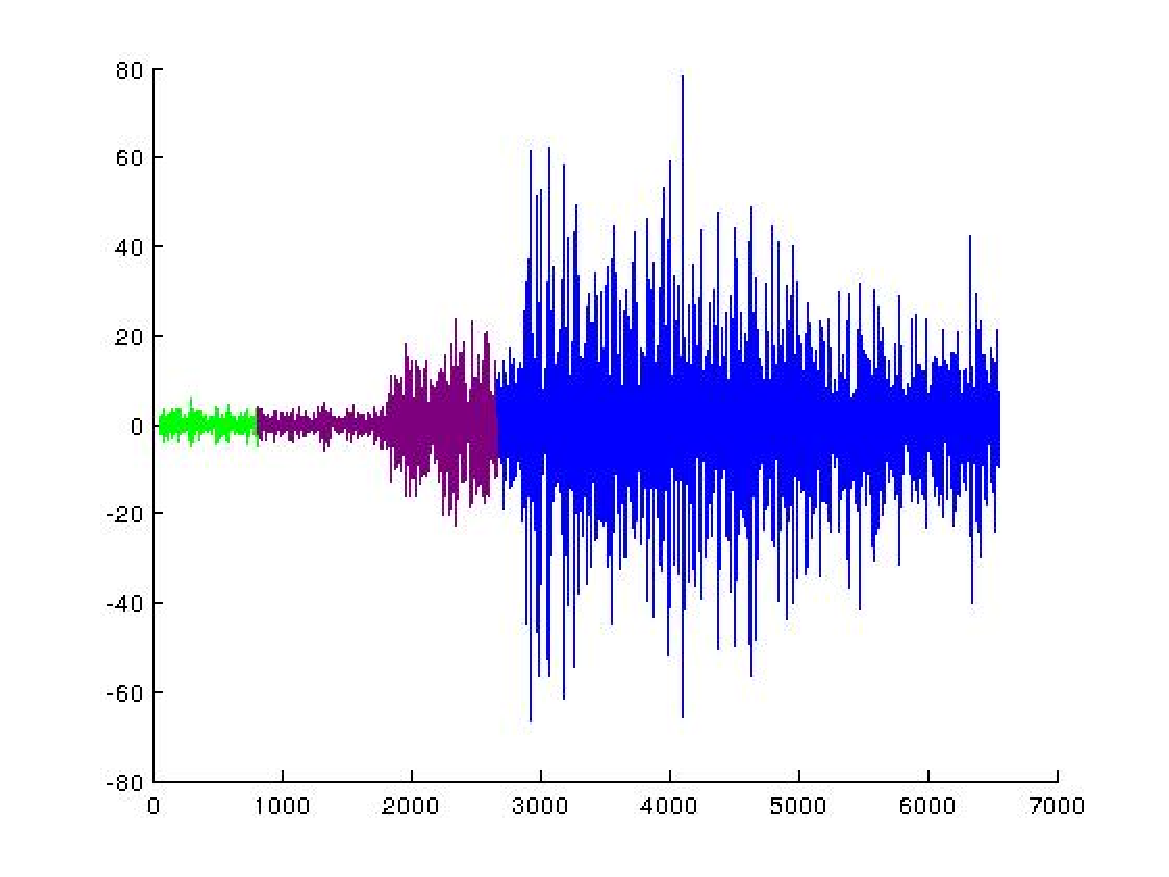
\includegraphics[height=4.7cm]{fig/R17F8S3P4.pdf}
		\end{column}
		\begin{column}{0.5\textwidth}
			Segmentation of time series with respect to the variance
		\end{column}
	\end{columns}
\end{center}

\end{frame}

%%%%%%%%%%%%%%%%%%%%%%%%%%%%%%%%%%%%%%%%%%%%%%%%%%%%%%%%%%%%%%
\begin{frame} \frametitle{Example (I): Clustering}
\begin{itemize}
\item Data: points $(x_j)_{j=1,\ldots,n}$ in ${\mathbb R}^d$.
\item Aim: find (\& predict) clusters.
\item Model-based approach: let $z_j$ be the (unknown) cluster of $x_j$.\\
 $z_i=z_j \Rightarrow x_i$ and $x_j$ should have the same (conditional) distribution.
\end{itemize}
\begin{center}
\only<1>{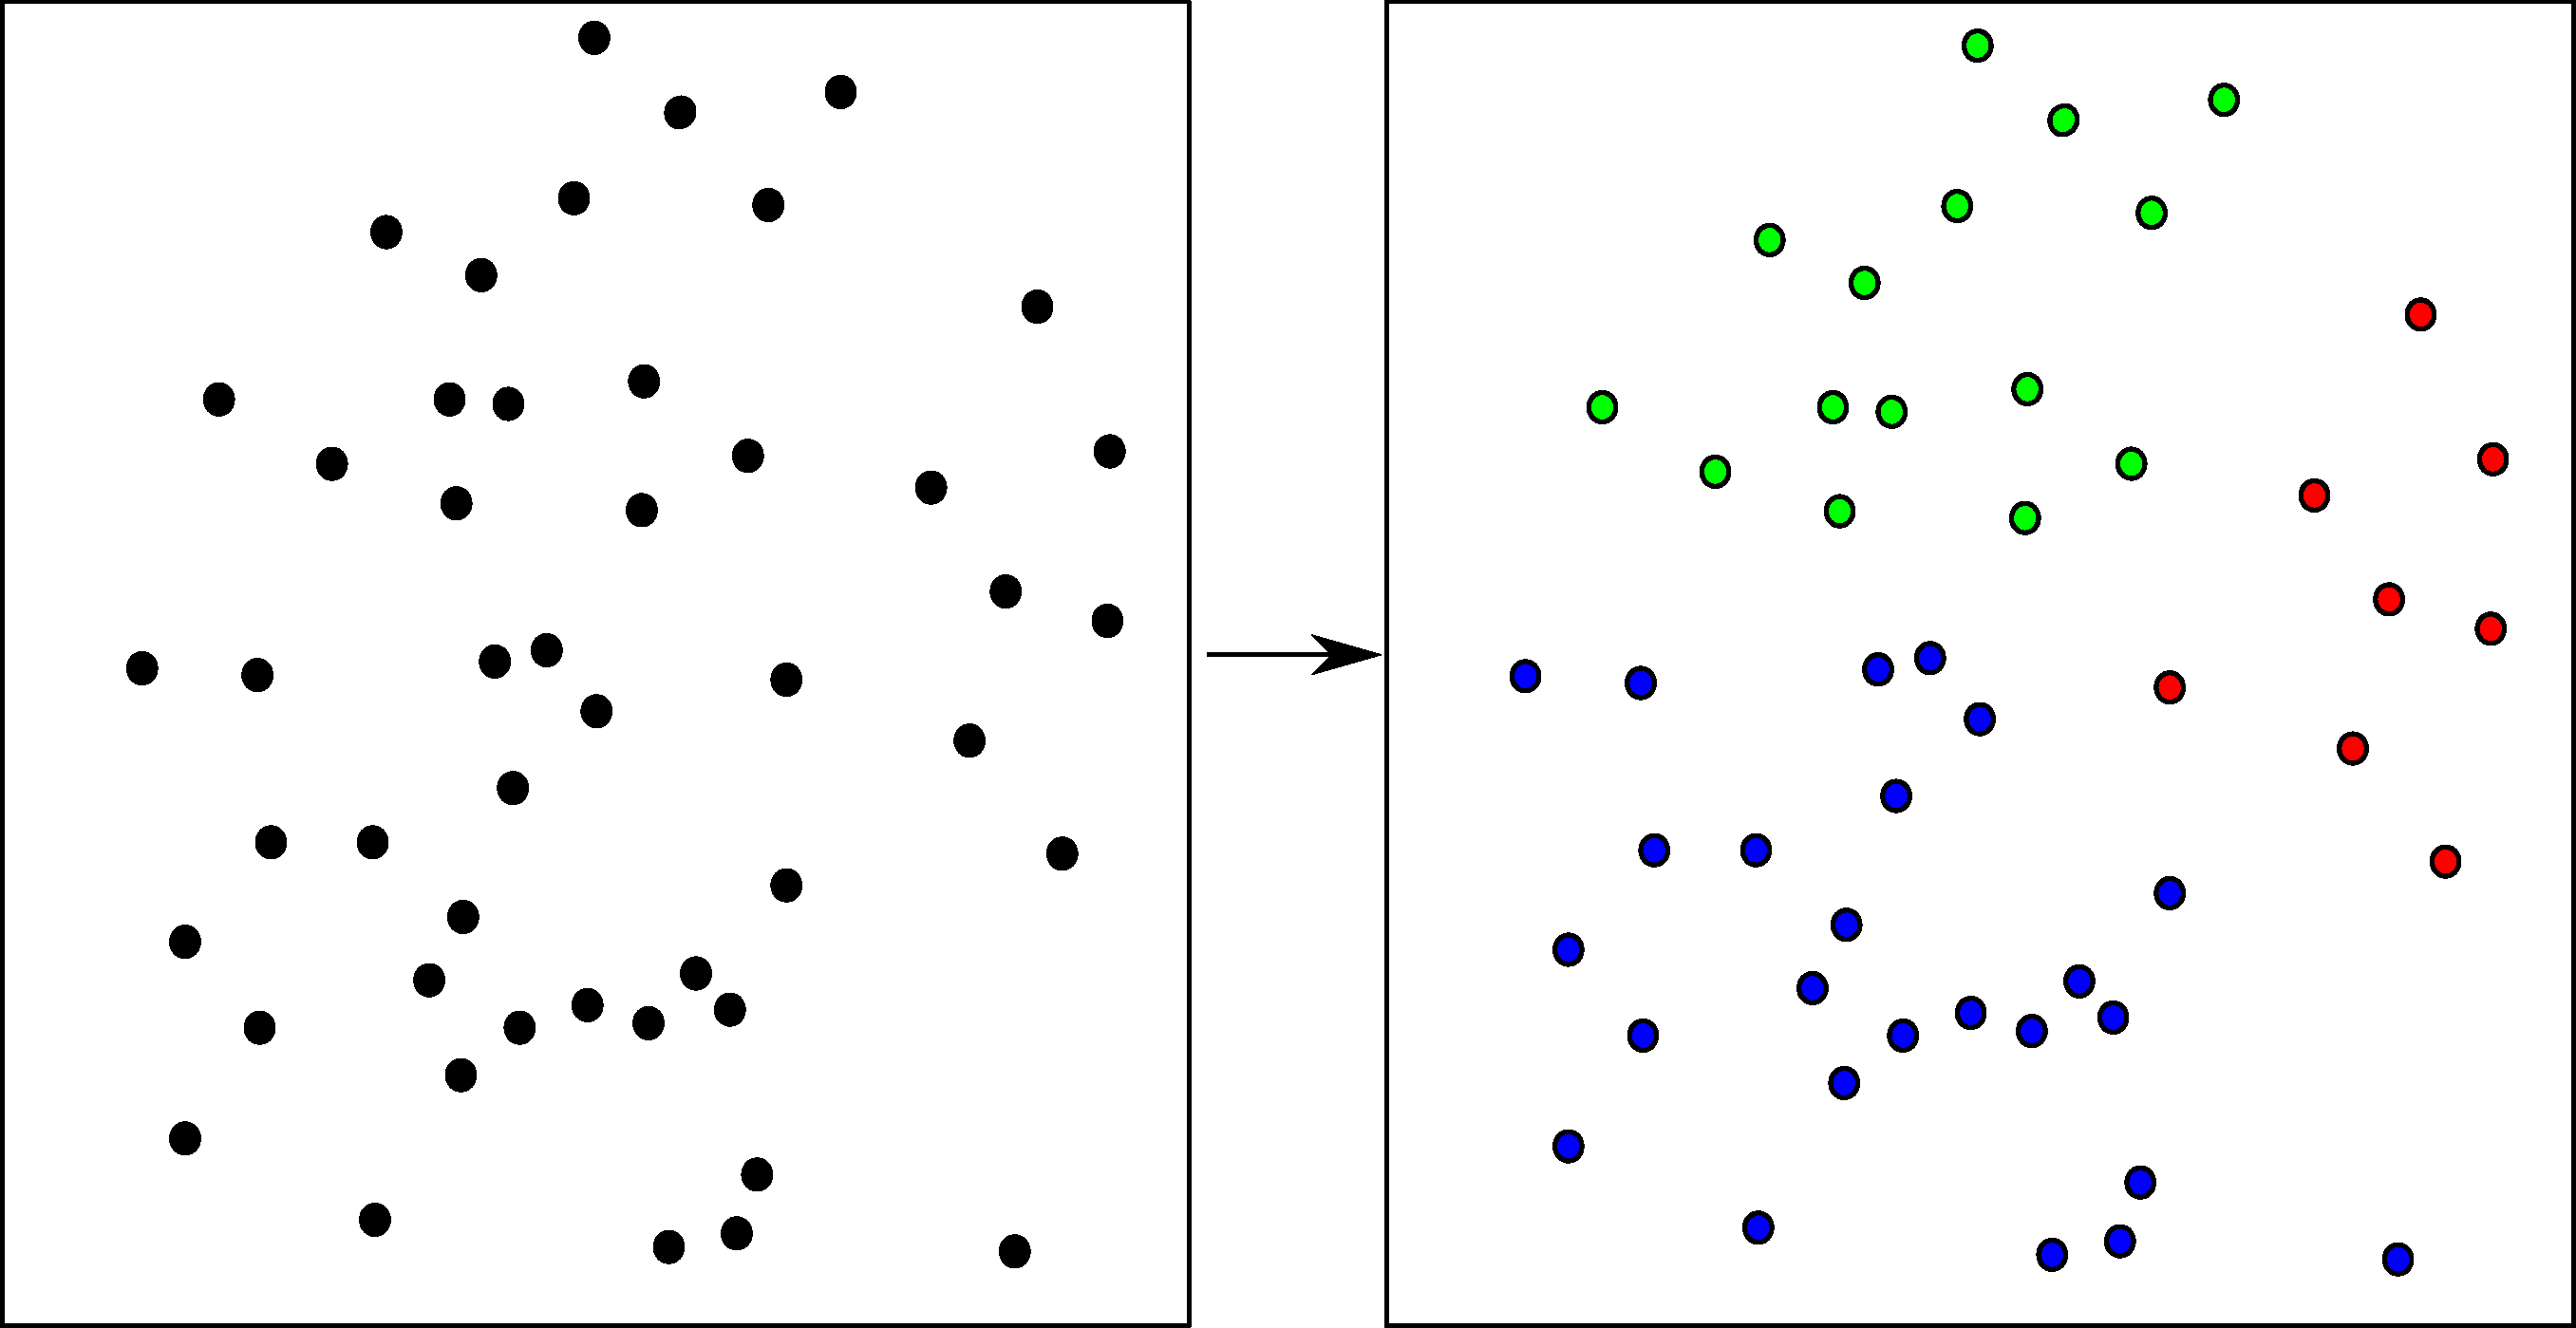
\includegraphics[height=4.5cm]{fig/clustering.pdf}}%
%\only<2>{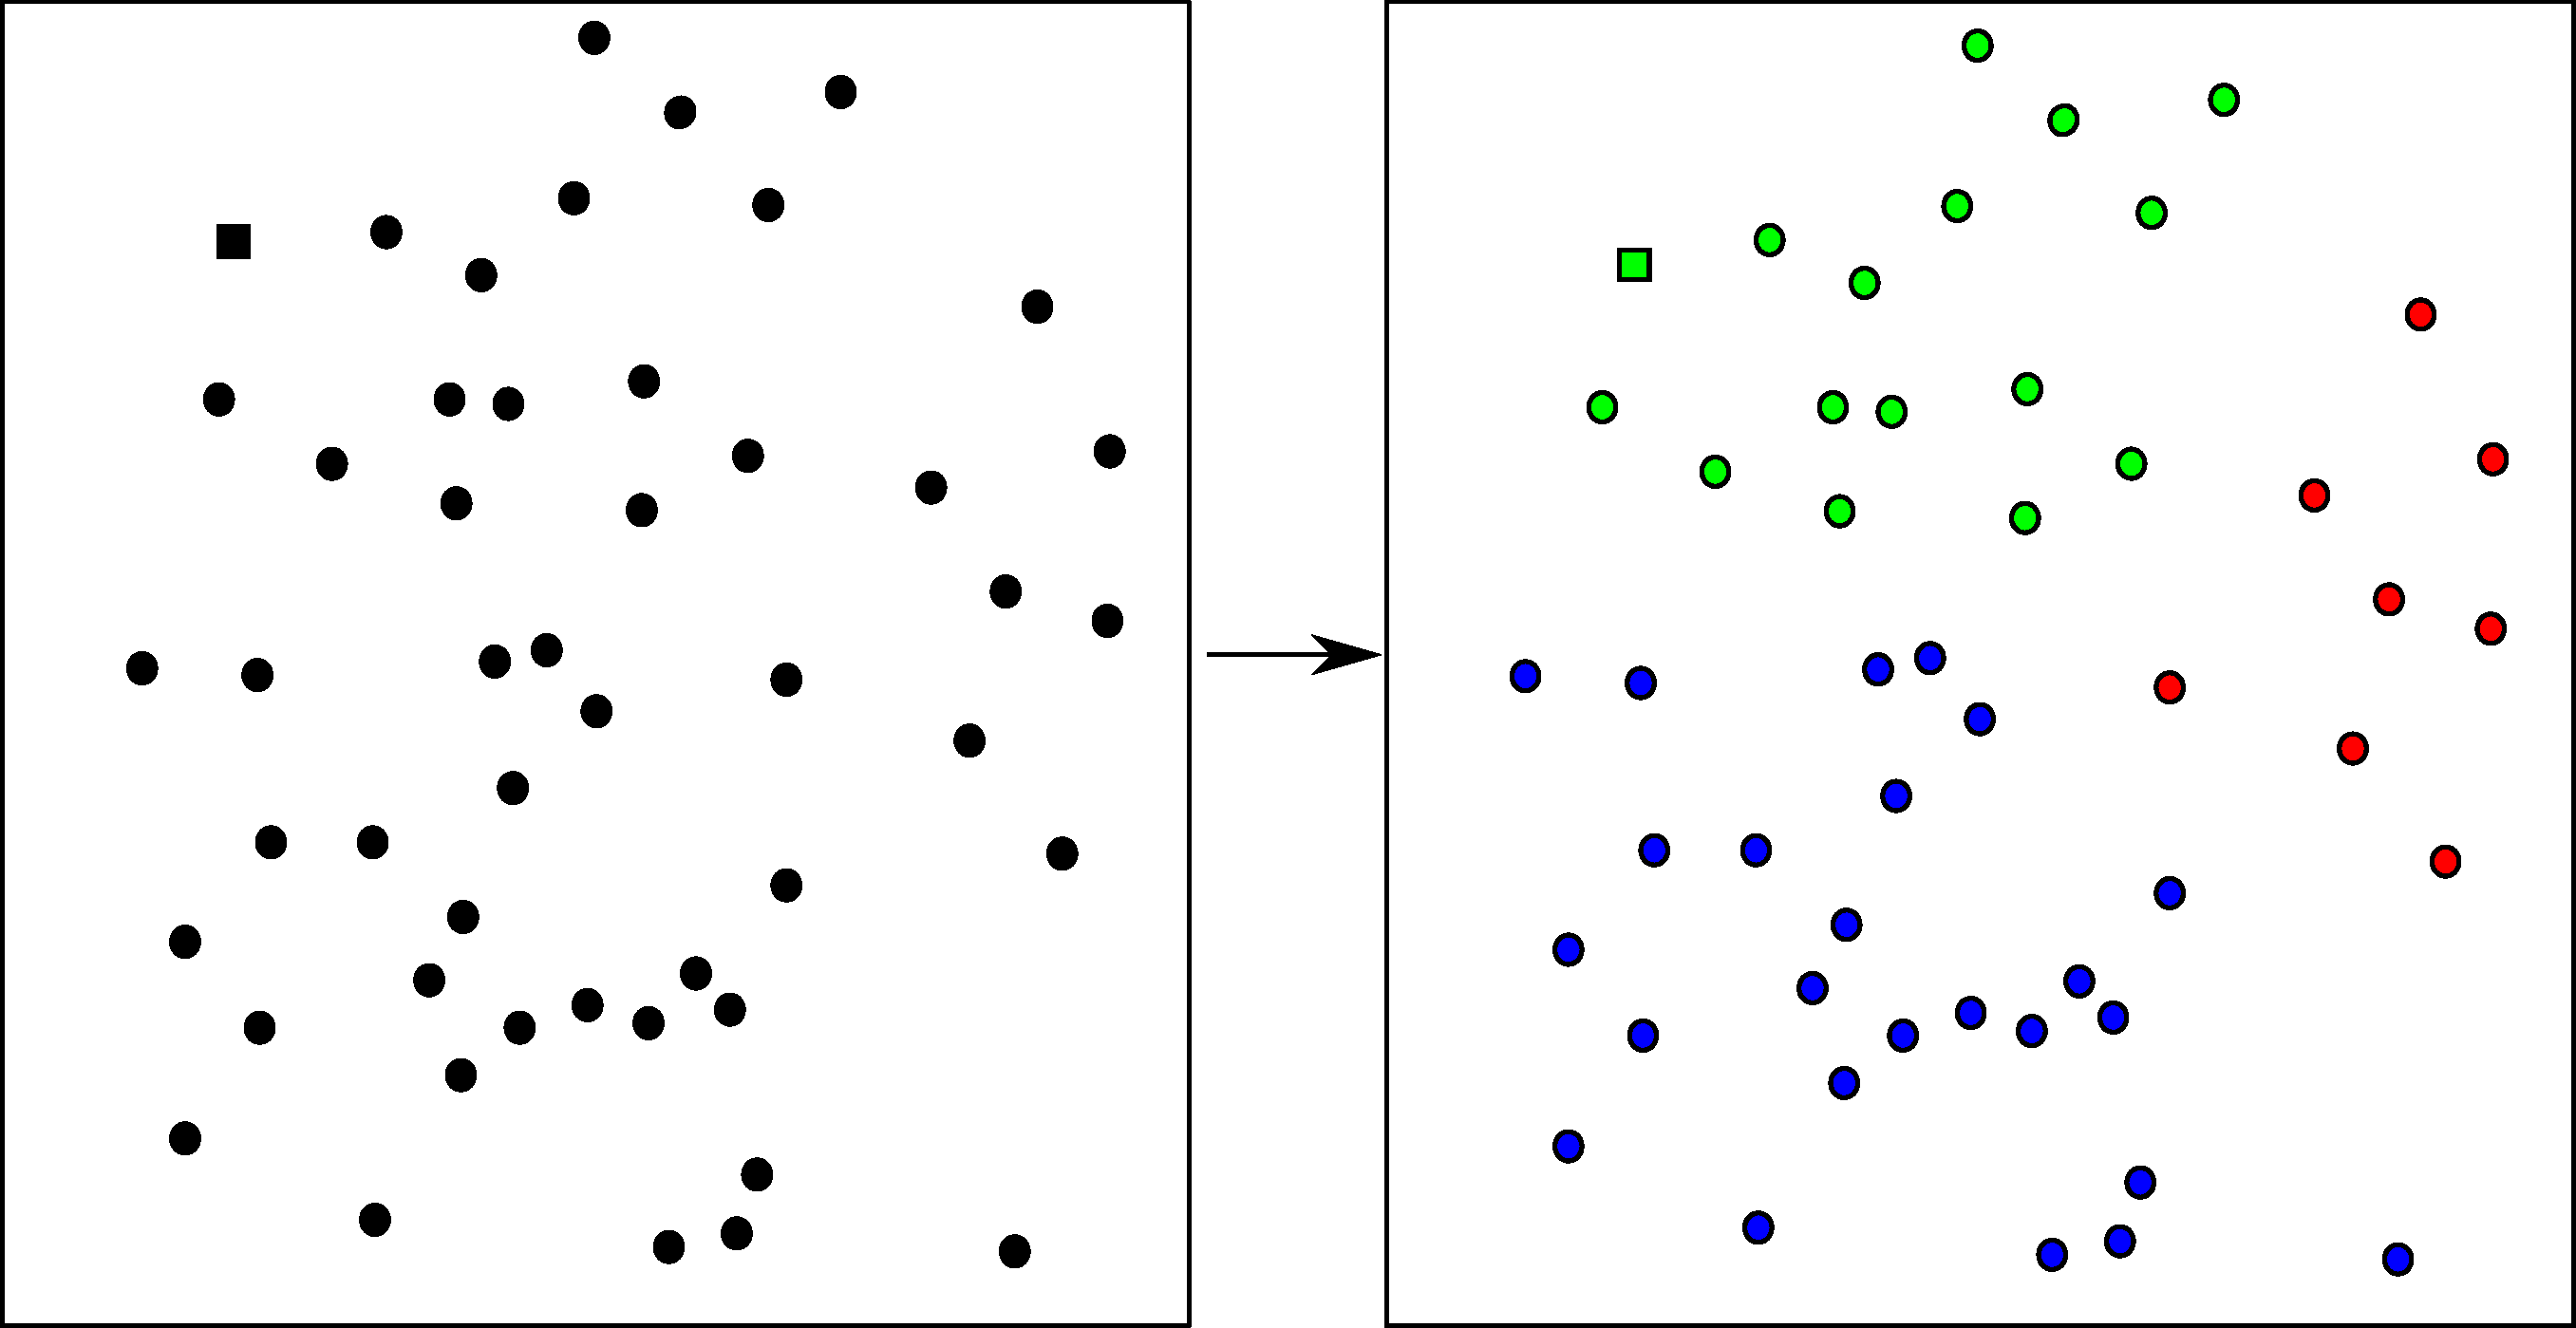
\includegraphics[height=4.5cm]{fig/clustering-1.pdf}}%
%\only<3>{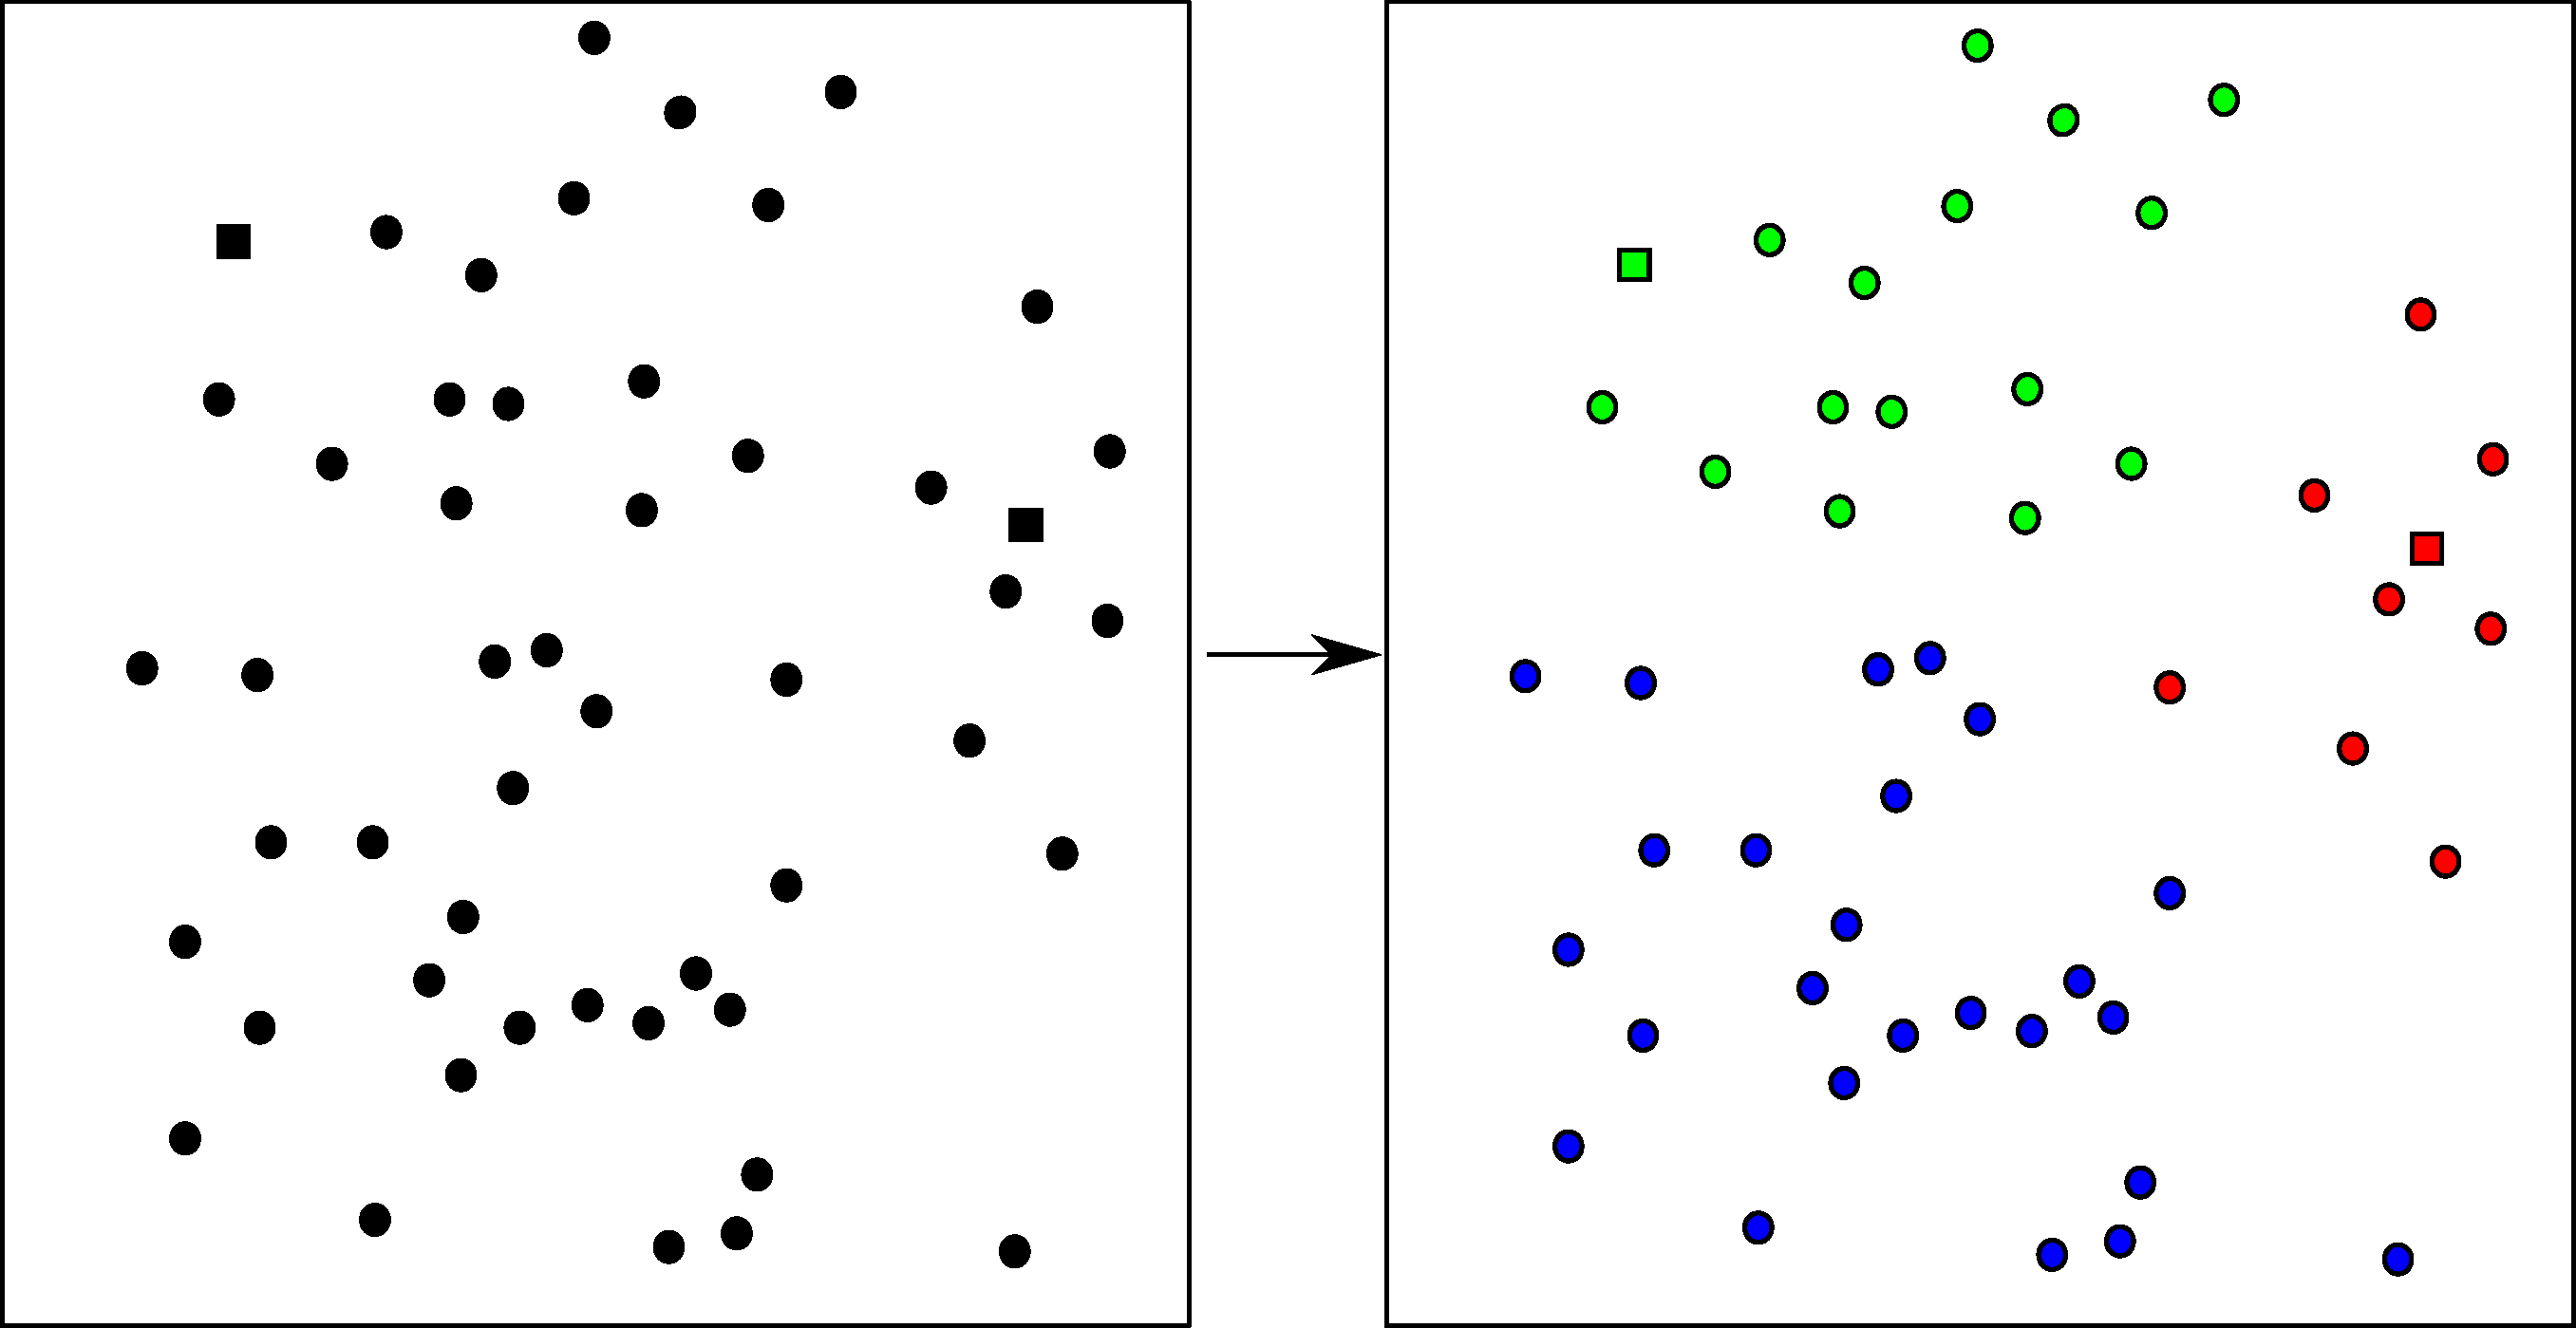
\includegraphics[height=4.5cm]{fig/clustering-2.pdf}}%
%\only<4>{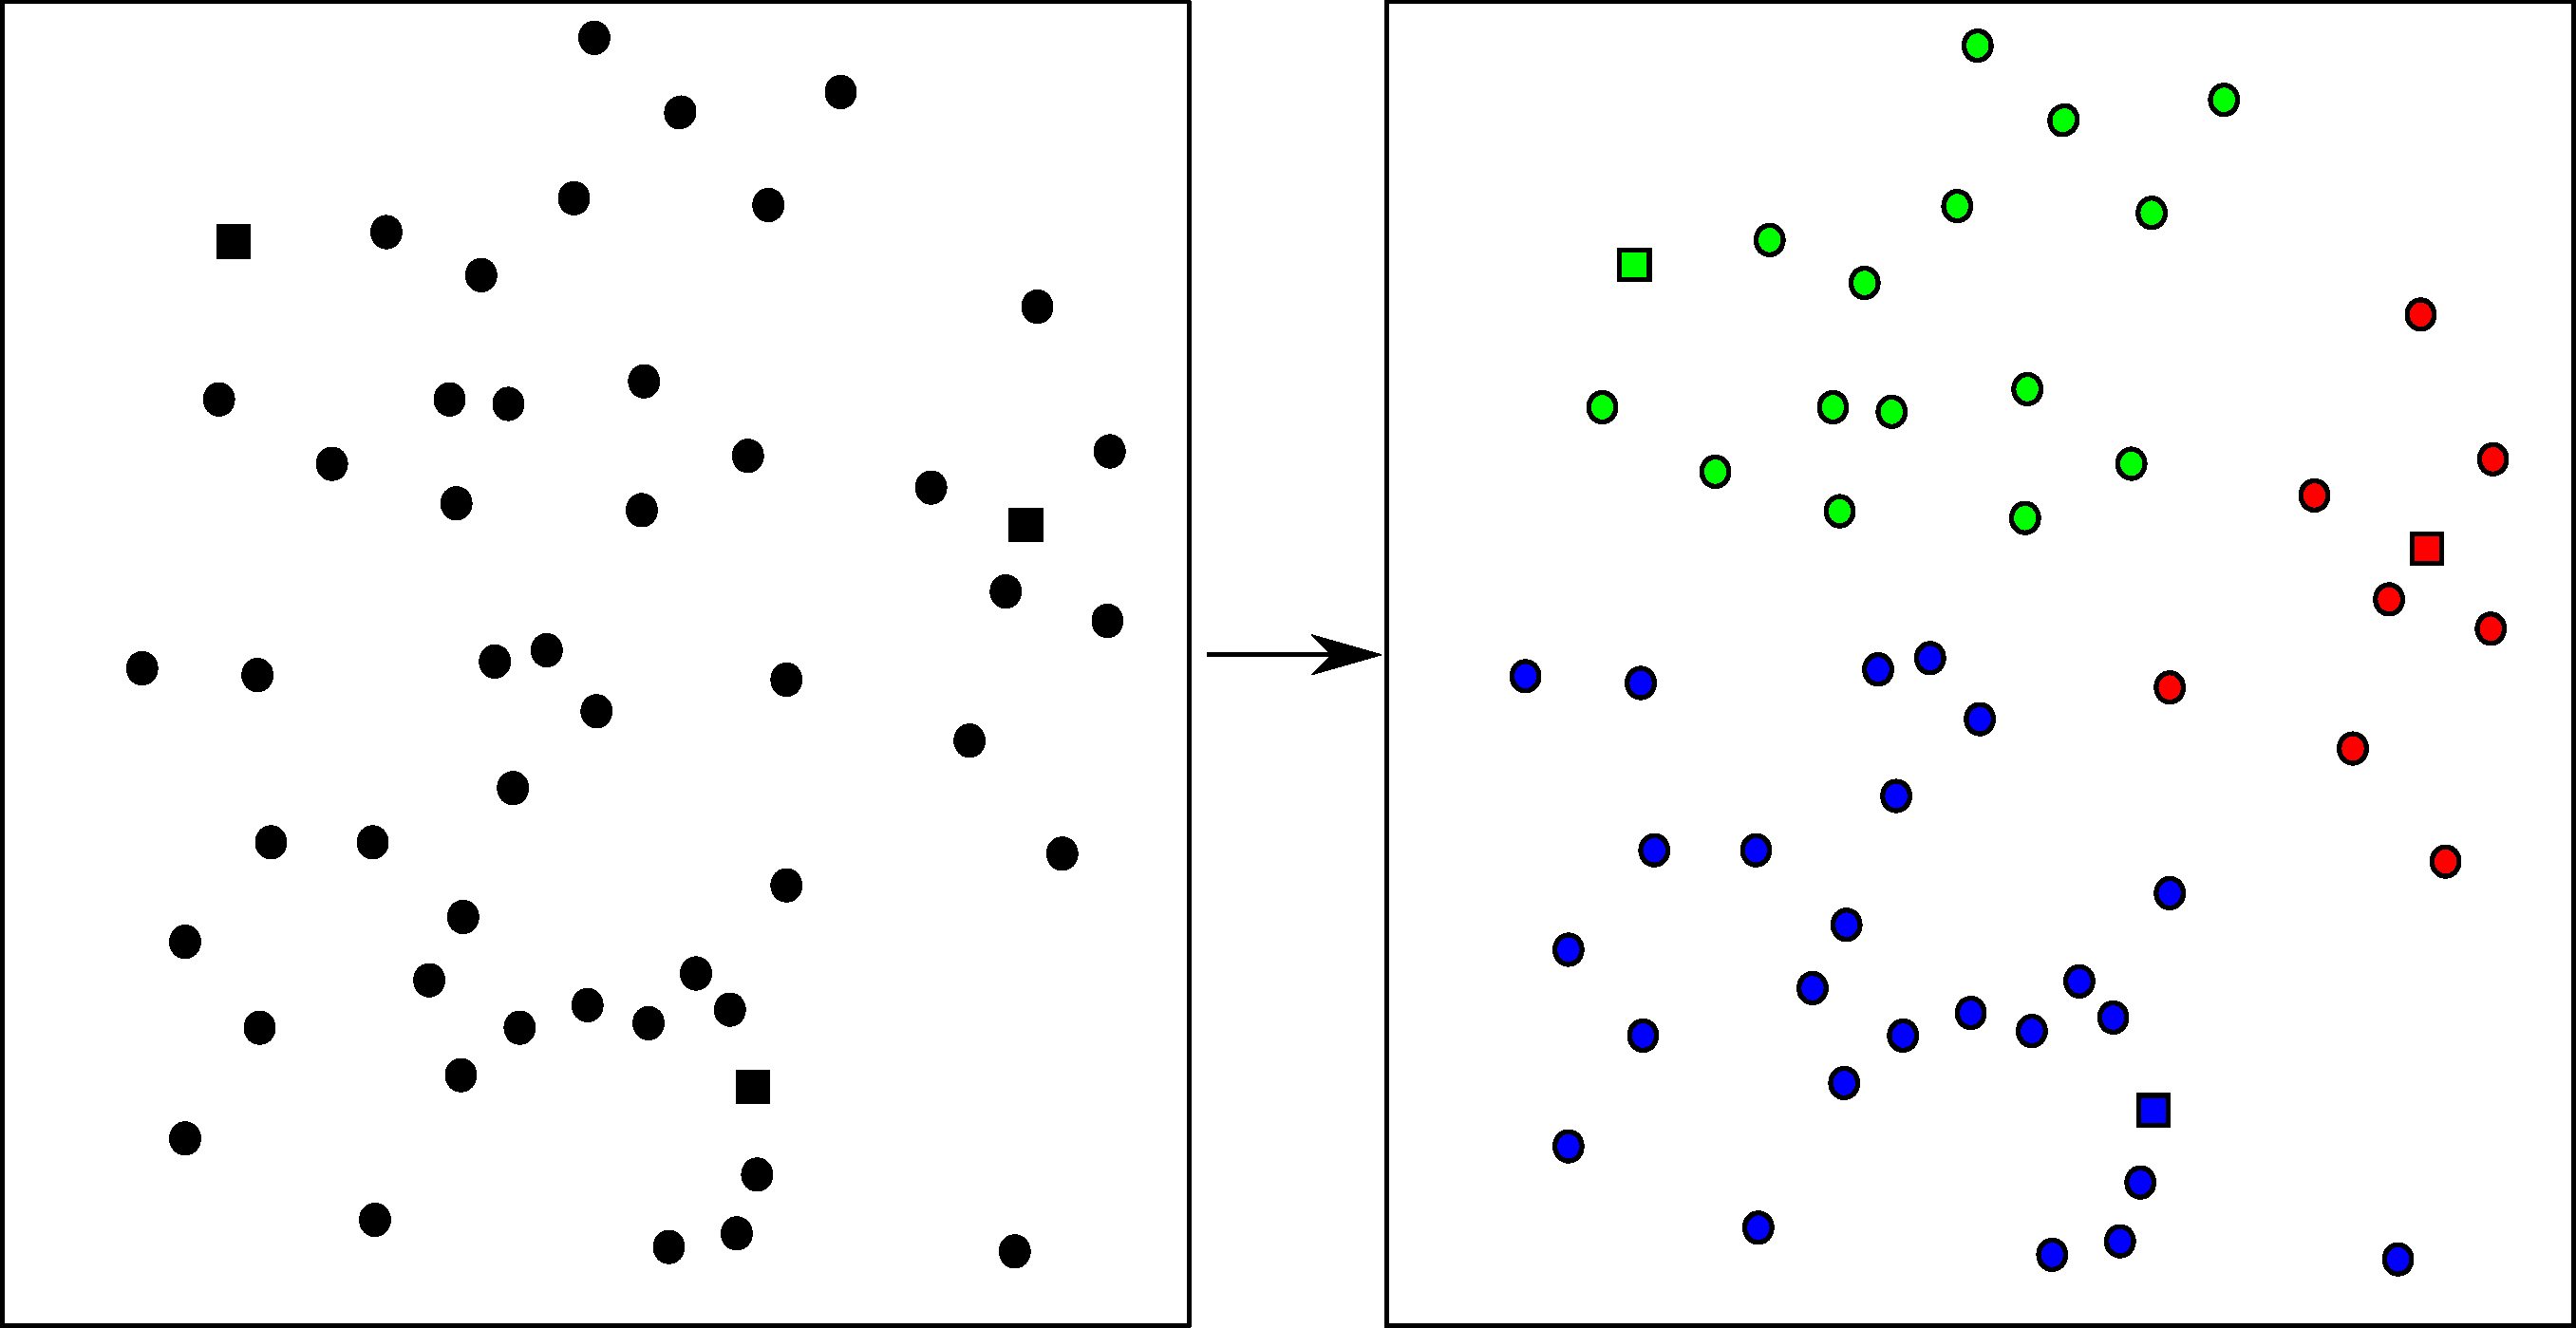
\includegraphics[height=4.5cm]{fig/clustering-3.pdf}}%
% $Z$ is an unknown / latent variable, useful for clustering. \\
% (e.g. $z=0 \rightarrow$ blue)
\end{center}
\end{frame}

%%%%%%%%%%%%%%%%%%%%%%%%%%%%%%%%%%%%%%%%%%%%%%%%%%%%%%%%%%%%%%
\begin{frame} \frametitle{Example (II): Dimensionality reduction}


	\begin{itemize}
	\item Raw data are high-dimensional descriptors.
	\item Difficult to mine patterns/visualize.
	\item Projection on the directions of maximum variance.
	\item What if for most or even every point $x_j$, some coordinates 
	 are missing?
	\item Probabilistic (i.e., model-based) PCA relies on a generative model to exploit partially observed / unknown data.
	\end{itemize}
	
	\begin{center}
% 		\begin{columns}
%             \begin{column}{.5\textwidth}
%                 \begin{align*}
%               -hyper      & x_i = W \gamma_i + \mu + \varepsilon_i\\
%                     & \text{with } W\in\RR^{D\times M}, M \ll D \\
%                     & \varepsilon_i \sim \MN(0, \sigma^2 I_D) \indep \gamma_i \sim \MN(0, I_M)
%                 \end{align*}
%             \end{column}
%             \begin{column}{.5\textwidth}
                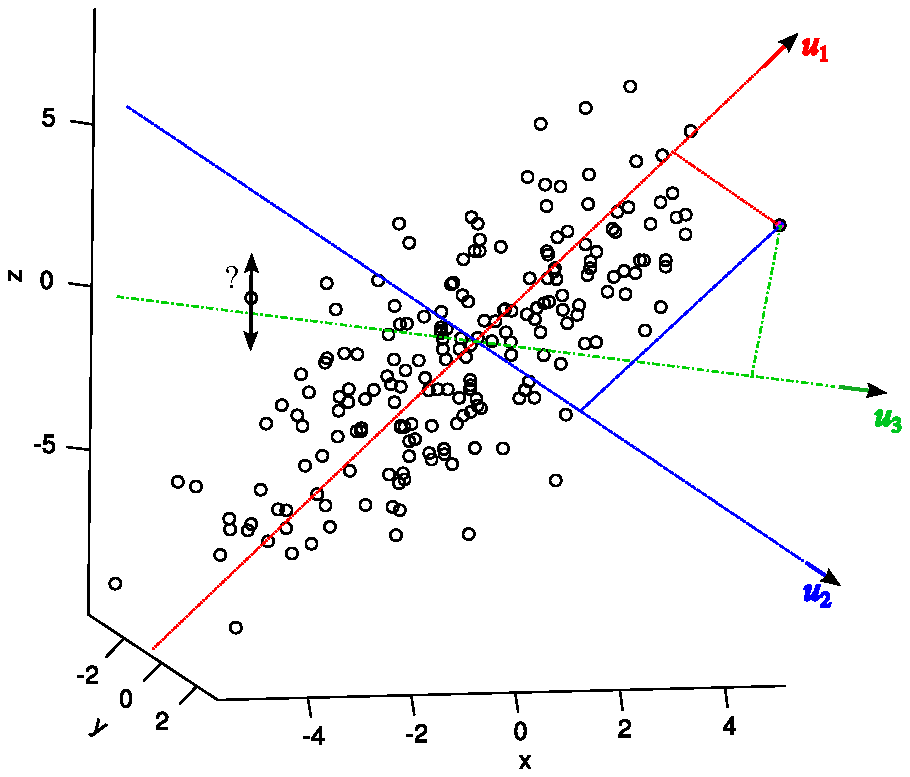
\includegraphics[height=4.4cm]{fig/ppca_cloud_axes.pdf}
%             \end{column}
% 		\end{columns}
	\end{center}
\end{frame}

%%%%%%%%%%%%%%\theexercise%%%%%%%%%%%%%%%%%%%%%%%%%%%%%%%%%%%%%%%%%%%%%%%%
\begin{frame} \frametitle{Example (III): Analysis of sequential data}
	\begin{itemize}
		\item Special case of clustering with temporal dependencies
		\item Piecewise statistically invariant features with Markovian jumps
		\item {\bf Markovian}: it depends \underline{only} on a few close neighbors.
	\end{itemize}
	\begin{center}
		\begin{columns}[t]
			\column{.005\textwidth}
			\column{.995\textwidth}
			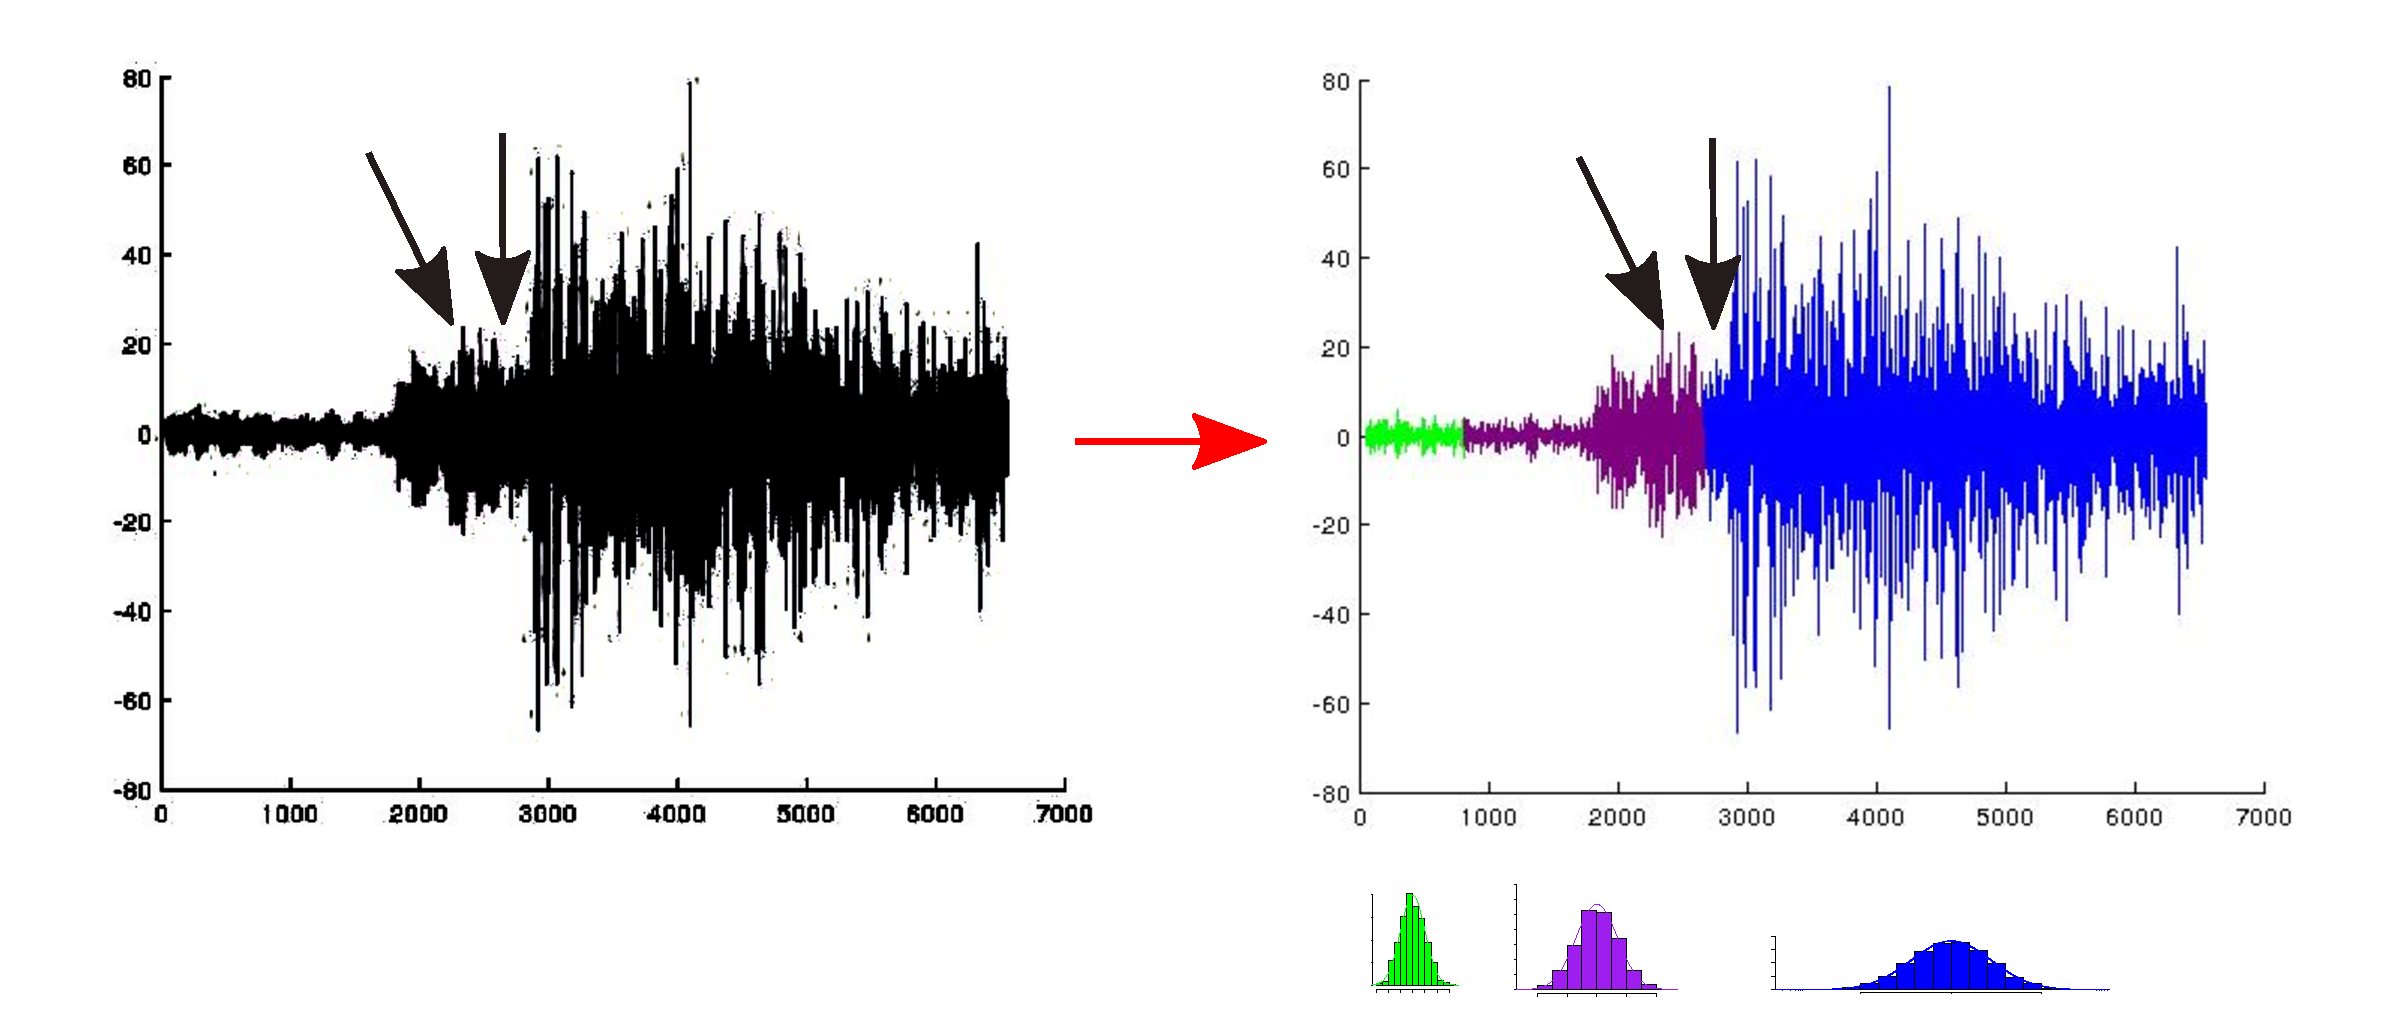
\includegraphics[height=4.4cm]{fig/hmm.pdf}
		\end{columns}
	\end{center}

\end{frame}

%%%%%%%%%%%%%%%%%%%%%%%%%%%%%%%%%%%%%%%%%%%%%%%%%%%%%%%%%%%%%%
\section{The multivariate Gaussian Distribution}
%%%%%%%%%%%%%%%%%%%%%%%%%%%%%%%%%%%%%%%%%%%%%%%%%%%%%%%%%%%%%%

%%%%%%%%%%%%%%%%%%%%%%%%%%%%%%%%%%%%%%%%%%%%%%%%%%%%%%%%%%%%%%
\begin{frame}{1D Gaussians}
 Let's recall the definition of the univariate Gaussian distribution, for $x\in\mathbb{R}$:
\[p(x) = \mathcal{N}(x;\mu,\nu) = \frac{1}{\sqrt{2\pi\nu}}\exp\Big(-\frac{(x-\mu)^2}{2\nu}\Big),\]
\begin{itemize}
 \item $\mu=\mathbb{E}_{\mathcal{N}(x;\mu,\nu)}\{x\}\in\mathbb{R}$ is the mean.
 \item $\nu=\mathbb{E}_{\mathcal{N}(x;\mu,\nu)}\{(x-\mu)^2\}\in\mathbb{R}^{+}$ is the variance.
\end{itemize}\vspace{3mm}
\pause
\remark{definition-expectation}{We will often use the \textbf{expectation} of a function $f$ of a random variable $x$ w.r.t.\ the probability density function $p(x)$, and denote it by:
\[
 \mathbb{E}_{p(x)}\{f(x)\} = \int_{\mathcal{X}} f(x)p(x)\textrm{d}x,
\]
where $\mathcal{X}$ is the domain of the random variable $x$.}
\end{frame}


\begin{frame}{1D Gaussians: ML estimators}
And of its ML estimators for a set of $N$ samples $X=\{x_1,\ldots,x_N\}$:
\[\mathcal{L}(\mu,\nu|X) = \sum_{n=1}^N \log \mathcal{N}(x_n;\mu,\nu)\]
\exercise{ml-uni-gaussian}{Prove that the maximum likelihood estimators are:
\[ \mu^* = \frac{1}{N}\sum_{n=1}^N x_n \qquad \nu^*=\frac{1}{N}\sum_{n=1}^N (x_n-\mu^*)^2.\]}\vspace{3mm}
\underline{Hint}: Compute $\displaystyle\frac{\partial\mathcal{L}}{\partial\mu}$ and $\displaystyle\frac{\partial\mathcal{L}}{\partial\nu}$ knwoing that $ \log \mathcal{N}(x;\mu,\nu) = -\frac{1}{2}\left(\log(2\pi\nu) + \frac{(x-\mu)^2}{\nu}\right) $.
\end{frame}

%%%%%%%%%%%%%%%%%%%%%%%%%%%%%%%%%%%%%%%%%%%%%%%%%%%%%%%%%%%%%%
\begin{frame}{Proof}
 \begin{align*}
  \mathcal{L}(\mu,\nu|X) &= \sum_{n=1}^N \log \mathcal{N}(x_n;\mu,\nu) \\
  &= -\frac{1}{2}\sum_{n=1}^N \log(2\pi\nu) + \frac{(x_n-\mu)^2}{\nu} \\
  &= -\frac{1}{2}\left(N\log(2\pi\nu) + \frac{1}{\nu}\sum_{n=1}^N(x_n-\mu)^2\right)
 \end{align*}
And hence:
\[\frac{\partial\mathcal{L}}{\partial\mu}=\frac{1}{\nu}\sum_{n=1}^N(x_n-\mu) \qquad \frac{\partial\mathcal{L}}{\partial\nu}=-\frac{N}{2\nu} + \frac{1}{2\nu^2}\sum_{n=1}^N(x_n-\mu)^2\]
By setting the derivatives to 0, we obtain the sought result.
\end{frame}
 
%%%%%%%%%%%%%%%%%%%%%%%%%%%%%%%%%%%%%%%%%%%%%%%%%%%%%%%%%%%%%%
\begin{frame}{Multivariate Gaussian distribution}
Trivial extension: consider each dimension independently.
 \[p(\mathbf{x}) = \mathcal{N}(\mathbf{x};\bs{\mu},\bs{\nu}) = \prod_{d=1}^D\frac{1}{\sqrt{2\pi\nu_d}}\exp\Big(-\frac{(x_d-\mu_d)^2}{2\nu_d}\Big),\]
{\small with $\mathbf{x}=(x_1,\ldots,x_D)\in\mathbb{R}^d$, $\bs{\mu}=(\mu_1,\ldots,\mu_D)\in\mathbb{R}^d$ and $\bs{\nu}=(\nu_1,\ldots,\nu_D)\in\mathbb{R}^{+}$.}
\begin{figure}
 \centering
 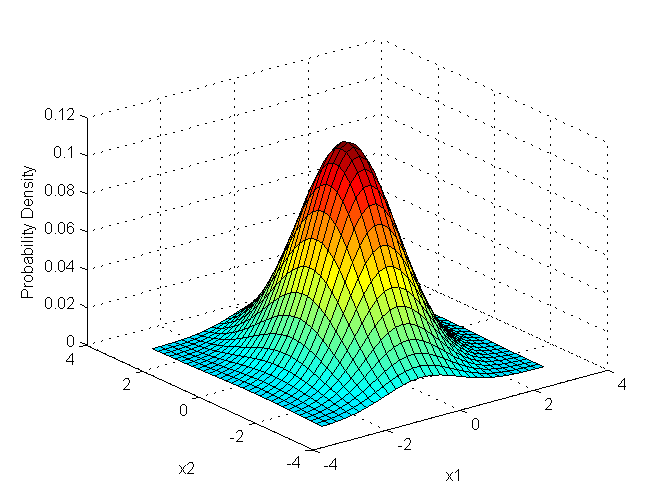
\includegraphics[width=0.5\textwidth]{fig/multivariate_gaussian}
\end{figure}
\exercise{ml-orth-gaussian}{Derive the maximum likelihood estimators for $\bs{\mu}$ and $\bs{\nu}$.} 
\end{frame}

%%%%%%%%%%%%%%%%%%%%%%%%%%%%%%%%%%%%%%%%%%%%%%%%%%%%%%%%%%%%%%
\begin{frame}{Multivariate Gaussian distribution (II)}
 By defining:
 \[\bs{\Sigma}=\textrm{diag}(\boldsymbol{\nu})=\left(\begin{array}{cccc}
 \nu_1 & 0 & \ldots & 0 \\
 0 & \nu_2 & \ldots & 0 \\
 \vdots & \vdots & \ddots & \vdots \\
 0 & 0 & \ldots & \nu_D
 \end{array}\right)
\]
 the density rewrites as:
 \[p(\mathbf{x}) = \mathcal{N}(\mathbf{x};\bs{\mu},\bs{\Sigma}) = \frac{1}{\sqrt{|2\pi\bs{\Sigma}|}}\exp\Big(-\frac{1}{2}(\bs{x}-\bs{\mu})^\top\bs{\Sigma}^{-1}(\bs{x}-\bs{\mu})\Big).\]
\exercise{matrix-form-equivalence-gaussian}{Prove it!}
\end{frame}

%%%%%%%%%%%%%%%%%%%%%%%%%%%%%%%%%%%%%%%%%%%%%%%%%%%%%%%%%%%%%%
\begin{frame}{Symmetric and positive definite matrices}
 \textbf{Question}: does it work for any matrix $\bs{\Sigma}$?\vspace{3mm}

 Only for \textit{symmetric} and \textit{positive definite} (s.p.d.) matrices.\vspace{3mm}
 
 \remark{positive-definite}{A $D\times D$ symmetric matrix $\bs{\Sigma}$ is \textbf{positive definite} if and only if $\bs{v}^\top\bs{\Sigma}\bs{v} > 0$, $\forall \bs{v}\neq \bs{0}$.}\vspace{3mm}
 \pause

 For the Gaussian distribution, this is intuitive, since the variance should be strictly positive in any direction:\vspace{-5mm}
 \begin{figure}
 \centering
 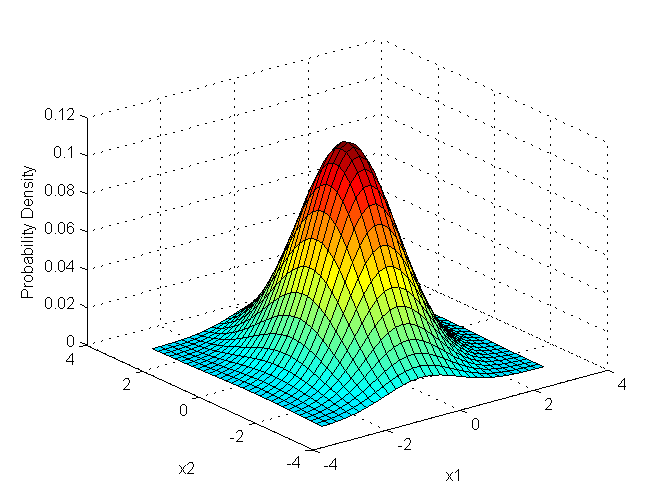
\includegraphics[width=0.5\textwidth]{fig/multivariate_gaussian}
\end{figure}
 \end{frame}

%%%%%%%%%%%%%%%%%%%%%%%%%%%%%%%%%%%%%%%%%%%%%%%%%%%%%%%%%%%%%%
\begin{frame}{Symmetric and positive definite matrices (II)}
    Let $\bs{\Sigma}$ be a s.p.d.\ matrix:
    \begin{itemize}
        \item All eigenvalues of $\bs{\Sigma}$ are ...?\pause\ Real and \pause strictly positive!
        \item The inverse of $\bs{\Sigma}$ is ...?\pause\ Symmetric and positive definite.
        \item How do we know that $\bs{\Sigma}^{-1}$ exists? \pause\ The determinant is the product of eigenvalues.
        \item We can write $\bs{\Sigma}=\bs{U}\bs{\Lambda}\bs{U}^\top$ with $\bs{\Lambda}$ diagonal and $\bs{U}$ orthogonal. Why?\pause
        \item So $\bs{\Lambda}$ contains eigenvalues and $\bs{U}$ contains eigenvectors (as columns).\pause
        \item Then, $\bs{\Sigma}^{-1} = \bs{U}\bs{\Lambda}^{-1}\bs{U}^\top$.
    \end{itemize}\vspace{3mm}
    \exercise{inv-pdf-matrix}{Prove that the inverse of a (symmetric) positive definite matrix always exists.}
\end{frame}
 
%%%%%%%%%%%%%%%%%%%%%%%%%%%%%%%%%%%%%%%%%%%%%%%%%%%%%%%%%%%%%%
\begin{frame}{Defining multivariate Gaussians}

\remark{def-mv-Gaussian}{Given a vector $\bs{\mu}\in\mathbb{R}^D$ and a s.p.d.\ matrix $\bs{\Sigma}\in\mathbb{R}^{D\times D}$, we can define the \textbf{multivariate Gaussian} distribution as:
\[
\mathcal{N}(\bs{x};\bs{\mu},\bs{\Sigma}) = \frac{1}{\sqrt{|2\pi\bs{\Sigma}|}}\exp\Big(-\frac{1}{2}(\bs{x}-\bs{\mu})^\top\bs{\Sigma}^{-1}(\bs{x}-\bs{\mu})\Big)
\]
}\vspace{3mm}

$\bs{\mu}$ and $\bs{\Sigma}$ are usually referred to as the \textit{mean vector} and the \textit{covariance matrix}, and they are defined as:
\[
\bs{\mu} = \mathbb{E}_{\mathcal{N}(\bs{x};\bs{\mu},\bs{\Sigma})}\{\mathbf{x}\} \qquad \bs{\Sigma} = \mathbb{E}_{\mathcal{N}(\bs{x};\bs{\mu},\bs{\Sigma})}\{(\mathbf{x}-\bs{\mu})(\mathbf{x}-\bs{\mu})^\top\}.
\]

\exercise{norm-mv-Gaussian}{Prove that the normalisation constant of a multivariate Gaussian distribution with covariance matrix $\bs{\Sigma}$ is $\sqrt{|2\pi\bs{\Sigma}|}$.}\vspace{3mm}
    
Jupyter Notebook!!!
\end{frame}

%%%%%%%%%%%%%%%%%%%%%%%%%%%%%%%%%%%%%%%%%%%%%%%%%%%%%%%%%%%%%%
\begin{frame}{Standard Gaussian and Affine Transforms}
 \remark{standard-gaussian}{The \textbf{standard multivariate Gaussian} is defined as the zero-mean and unit-variance Gaussian distribution:
\[
 \mathcal{N}(\mathbf{z};\mathbf{0},\mathbf{I}) = \frac{1}{(2\pi)^{D/2}}\exp\Big(-\frac{1}{2}\|\mathbf{z}\|^2\Big).
\]
}\vspace{2mm}

\exercise{mv-gaussian-linear-construction}{Let us consider the case where $\mathbf{z}$ follows a standard multivariate Gaussian distribution, and we define $\mathbf{x}=\mathbf{A}\mathbf{z}+\bs{\mu}$ with $\mathbf{A}\in\mathbb{R}^{D\times D}$ being an invertible matrix ($|\mathbf{A}|\neq 0$). Prove that:
\[
 p(\mathbf{x}) = \mathcal{N}(\bs{x};\bs{\mu},\bs{\Sigma}), \quad \text{with} \quad \bs{\Sigma} = \mathbf{A}\mathbf{A}^\top.
\]
}
\end{frame}

%%%%%%%%%%%%%%%%%%%%%%%%%%%%%%%%%%%%%%%%%%%%%%%%%%%%%%%%%%%%%%
\begin{frame}{More on Multivariate Gaussians}
    What are the level curves of the Gaussian p.d.f.?
    \[\mathcal{C}_\lambda = \{\bs{x}|\mathcal{N}(\bs{x};\bs{\mu},\bs{\Sigma})=\lambda\}.\]
    \pause
    \begin{columns}
     \begin{column}{0.5\textwidth}
     \small
    \begin{itemize}
     \item Empty set for $\lambda<0$.
     \item $\mathcal{C}_0=\{\bs{\mu}\}$.
     \item $\mathcal{C}_\lambda$? \pause\ An ellipsoid with center $\bs{\mu}$ with axis given by the columns of $\bs{U}$ and axis length given by the elements in $\bs{\Lambda}$, where $\bs{\Sigma}=\bs{U}\bs{\Lambda}\bs{U}^\top$.
    \end{itemize}
     \end{column}
     \begin{column}{0.5\textwidth}
      \centering
      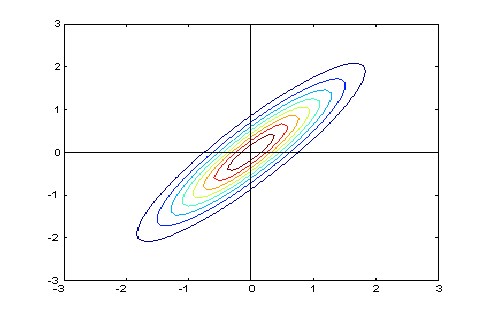
\includegraphics[width=\textwidth]{fig/ellipsoids.png}
     \end{column}

    \end{columns}

\end{frame}

%%%%%%%%%%%%%%%%%%%%%%%%%%%%%%%%%%%%%%%%%%%%%%%%%%%%%%%%%%%%%%
\begin{frame}{ML for multivariate Gaussians}
\exercise{ml-estimators-mv-gaussian}{Prove that the ML estimators of the multivariate Gaussian are:
\[
\bs{\mu}^*=\frac{1}{N}\sum_{n=1}^N\bs{x}_n\qquad \bs{\Sigma}^* = \frac{1}{N}\sum_{n=1}^N (\bs{x}_n-\bs{\mu}^*)(\bs{x}_n-\bs{\mu}^*)^\top.
\]
}\vspace{3mm}\pause

You will need to take derivatives w.r.t.\ matrices. Let $\bs{M}$ be a matrix, and $f(\bs{M})$ and function of that matrix (e.g.\ trace, ...). One can consider $\frac{\partial f}{\partial\bs{M}}$.\vspace{3mm}
 
 Examples of matrix derivative formulae useful to derive the ML estimate of multivariate Gaussians:
 \[\frac{\partial \textrm{Tr}(\bs{M}\bs{A})}{\partial\bs{M}}=\bs{A}^\top \qquad \frac{\partial \textrm{Tr}(\bs{B}^\top\bs{M}^\top\bs{C}\bs{M}\bs{B})}{\partial\bs{M}}=\bs{C}^\top\bs{M}\bs{B}\bs{B}^\top+\bs{C}\bs{M}\bs{B}\bs{B}^\top\]
 
 \[\frac{\partial \log|\bs{M}|}{\partial\bs{M}}=(\bs{M}^{-1})^\top \qquad [\textrm{Tr}(\bs{A}\bs{B}\bs{C}) = \textrm{Tr}(\bs{B}\bs{C}\bs{A}) = \textrm{Tr}(\bs{C}\bs{A}\bs{B})]\]
 

\end{frame}

\begin{frame}{Gaussian Completion: Shape is All You Need}
 \remark{shape-gaussians}{Developing multivariate Gaussian distribution, we observe that only two terms depend on $\mathbf{x}$ (quadratic and linear):
\[ 
\mathcal{N}(\bs{x};\bs{\mu},\bs{\Sigma}) \stackrel{\mathbf{x}}{\propto} \exp\Big(-\frac{1}{2}\bs{x}^\top\bs{\Sigma}^{-1}\bs{x} + \bs{x}^\top\bs{\Sigma}^{-1}\bs{\mu}\Big).
\]
{\small ($\stackrel{\mathbf{x}}{\propto}$ means that is proportional up to a constant that does NOT depend on $\mathbf{x}$)}
}\vspace{3mm}\pause
\exercise{gaussian-completion}{Prove that given a s.p.d.\ matrix $\bs{\Omega}$ and a vector $\mathbf{m}$:
\[
 p(\mathbf{x}) \stackrel{\mathbf{x}}{\propto} \exp\Big(-\frac{1}{2}\mathbf{x}^\top\bs{\Omega}\mathbf{x} + \mathbf{x}^\top\mathbf{m}\Big) \Rightarrow p(\mathbf{x})=\mathcal{N}(\bs{x};\bs{\mu},\bs{\Sigma})
\]
with:
\[
 \bs{\Sigma} = \bs{\Omega}^{-1} \qquad \qquad \bs{\mu} = \bs{\Sigma}\mathbf{m} = \bs{\Omega}^{-1}\mathbf{m}.
\]
}\vspace{3mm}

More on multivariate Gaussians in Chapter~\ref{notes-ch:ppca}.

\end{frame}

%%%%%%%%%%%%%%%%%%%%%%%%%%%%%%%%%%%%%%%%%%%%%%%%%%%%%%%%%%%%%%
\section{Latent Variables and Conditional Independence}
%%%%%%%%%%%%%%%%%%%%%%%%%%%%%%%%%%%%%%%%%%%%%%%%%%%%%%%%%%%%%%

%%%%%%%%%%%%%%%%%%%%%%%%%%%%%%%%%%%%%%%%%%%%%%%%%%%%%%%%%%%%%%
\begin{frame}{What is a model?}
What does it mean to \textit{model} the relationship between two variables?\vspace{3mm}
 \begin{columns}
  \begin{column}{0.08\textwidth}%
   
\includegraphics[width=0.8\textwidth]{fig/simple-model.pdf}
  \end{column}%
  \begin{column}{0.9\textwidth}
   \begin{itemize}
    \item \textit{We choose} the nature of $\bs{z}$ \& $\bs{x}$: cont./discrete, bounded, ...
    \item \textit{We choose} the \textcolor{green}{dependencies}, i.e.\ $p(\bs{x},\bs{z})=p(\bs{x}|\bs{z})p(\bs{z})$.
    \item \textit{We choose} the \textcolor{red}{prior distribution} $p(\bs{z})$.
    \item \textit{We choose} the \textcolor{blue}{likelihood distribution} $p(\bs{x}|\bs{z})$.
   \end{itemize}
  \end{column}
 \end{columns}
 \vspace{5mm}\pause
\only<2>{\remark{latent-variable-def}{There is an important difference between \textbf{observed} and \textbf{latent} or hidden variables. Observed variables are measured, and latent variables are quantities that cannot be measured directly.}}
\only<3>{\remark{classical-questions}{In models with latent variables, we study the \textbf{marginal distribution} of $\mathbf{x}$ (left) and the \textbf{posterior distribution} of $\mathbf{z}$ given $\mathbf{x}$ (right):
\[
p(\mathbf{x}) = \displaystyle\int_{\cal Z} p(\mathbf{x}|\mathbf{z})p(\mathbf{z}) \textrm{d}\mathbf{z} \qquad\qquad  
p(\mathbf{z}|\mathbf{x}) = \displaystyle\frac{p(\mathbf{x}|\mathbf{z})p(\mathbf{z})}{p(\mathbf{x})}
\]
}}
\end{frame}

%%%%%%%%%%%%%%%%%%%%%%%%%%%%%%%%%%%%%%%%%%%%%%%%%%%%%%%%%%%%%%
\begin{frame}{Example: Gaussian mixture model}
  \begin{columns}
  \begin{column}{0.08\textwidth}%
   
\includegraphics[width=0.8\textwidth]{fig/simple-model-black.pdf}
  \end{column}%
  \begin{column}{0.9\textwidth}
   \begin{itemize}
    \item The nature: $z$ is discrete \& bounded, $x$ is 1D \& continuous.
    \item The dependencies: $p(x,z)=p(x|z)p(z)$.
    \pause
    \item The distribution $p(z)$, $z\in\{1,\ldots,K\}$ is categorical:
    \[p(z=k) = \pi_k, \qquad \pi_k\geq 0,\; \sum_{k=1}^K \pi_k = 1.\]
    \pause
    \item The distribution $p(x|z)$ is Gaussian:
    \[p(x|z=k) = {\cal N}(x;\mu_k,\nu_k) = \frac{1}{\sqrt{2\pi\nu_k}}\exp\Big(-\frac{(x-\mu_k)^2}{2\nu_k}\Big)\]
    with $\mu_k\in\mathbb{R}$ and $\nu_k>0$, $\forall k$.
   \end{itemize}
  \end{column}
 \end{columns}
\end{frame}

%%%%%%%%%%%%%%%%%%%%%%%%%%%%%%%%%%%%%%%%%%%%%%%%%%%%%%%%%%%%%%
\begin{frame}{Likelihood and GMM posteriors}
\exercise{1d-gmm-marginal}{Prove that the GMM marginal writes:
\[ 
p(x) = \sum_{k=1}^K \pi_k \frac{1}{\sqrt{2\pi\nu_k}}\exp\Big(-\frac{(x-\mu_k)^2}{2\nu_k}\Big).
\]
}\vspace{3mm}

\exercise{1d-gmm-posterior}{Prove the GMM posterior writes:
\[
 p(z=k|x) = \frac{\pi_k \frac{1}{\sqrt{2\pi\nu_k}}\exp\Big(-\frac{(x-\mu_k)^2}{2\nu_k}\Big)}{\sum_{m=1}^K \pi_m \frac{1}{\sqrt{2\pi\nu_m}}\exp\Big(-\frac{(x-\mu_m)^2}{2\nu_m}\Big)}.
\]
}\vspace{3mm}

\underline{Hint}: Just write down what things are.\vspace{3mm}

More on this on the Chapter~\ref{notes-ch:gmm}.
\end{frame}

% %%%%%%%%%%%%%%%%%%%%%%%%%%%%%%%%%%%%%%%%%%%%%%%%%%%%%%%%%%%%%%
% \begin{frame}{Solution: likelihood and GMM posteriors}
%  The \textbf{likelihood}: $p(x) = \displaystyle\int_{\cal Z} p(x|z)p(z) \textrm{d}z \pause= \displaystyle\sum_{k=1}^K p(x|Z=k)p(Z=k)$.\pause
%  
%  And then we replace:
%  \[p(x) = \sum_{k=1}^K \pi_k \frac{1}{\sqrt{2\pi\nu_k}}\exp\Big(-\frac{(x-\mu_k)^2}{2\nu_k}\Big) \]\pause
%  The \textbf{posterior}:
%  \[p(Z=k|x) = \frac{\pi_k \frac{1}{\sqrt{2\pi\nu_k}}\exp\Big(-\frac{(x-\mu_k)^2}{2\nu_k}\Big)}{\sum_{m=1}^K \pi_m \frac{1}{\sqrt{2\pi\nu_m}}\exp\Big(-\frac{(x-\mu_m)^2}{2\nu_m}\Big)}\]
%  
%  More on this on the GMM chapter!!!
% \end{frame}

%%%%%%%%%%%%%%%%%%%%%%%%%%%%%%%%%%%%%%%%%%%%%%%%%%%%%%%%%%%%%%
\subsection{Conditional Independence}
%%%%%%%%%%%%%%%%%%%%%%%%%%%%%%%%%%%%%%%%%%%%%%%%%%%%%%%%%%%%%%
% 
% %%%%%%%%%%%%%%%%%%%%%%%%%%%%%%%%%%%%%%%%%%%%%%%%%%%%%%%%%%%%%%
% \begin{frame}{3-variable models: full}
% \begin{columns}
%   \begin{column}{0.12\textwidth}%
%    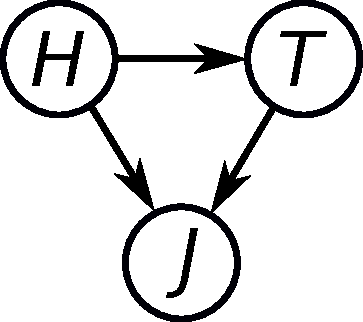
\includegraphics[width=1.2\textwidth]{fig/full-3var.pdf}
%   \end{column}%
%   \begin{column}{0.8\textwidth}
%     \begin{itemize}
%      \item The amount of sun $H$.
%      \item The amount of apple trees $T$.
%      \item The amount of juice $J$.
%     \end{itemize}
%   \end{column}
%  \end{columns}
%  \vspace{6mm}
%   The amount of trees clearly depends on the amount of sun.\\
%   The amount of juice depends on both sun and trees.\vspace{3mm}\\
%   \[p(j,t,h) = \only<1>{\alert{\text{You've got 3 minutes.}}}\only<2>{p(j|t,h)\;p(t|h)\;p(h)}\]
% \end{frame}
% 
% %%%%%%%%%%%%%%%%%%%%%%%%%%%%%%%%%%%%%%%%%%%%%%%%%%%%%%%%%%%%%%
% \begin{frame}{3-variable models: two-kids}
% \begin{columns}
%   \begin{column}{0.12\textwidth}%
%    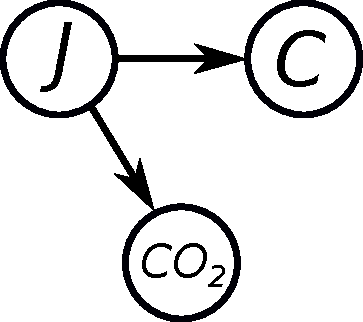
\includegraphics[width=1.2\textwidth]{fig/twokids-3var.pdf}
%   \end{column}%
%   \begin{column}{0.8\textwidth}
%     \begin{itemize}
%      \item The amount of juice $J$.
%      \item The amount of cider $C$.
%      \item The amount of $CO_2$.
%     \end{itemize}
%   \end{column}
%  \end{columns}
%  \vspace{6mm}
%   Both the amount of cider and $CO_2$ depend on $J$.\vspace{3mm}\\
%   \[p(co_2,c,j) = \only<1>{\alert{\text{You've got 3 minutes.}}}\only<2>{p(co_2|j)\;p(c|j)\;p(j)}\]
% \end{frame}
% 
% %%%%%%%%%%%%%%%%%%%%%%%%%%%%%%%%%%%%%%%%%%%%%%%%%%%%%%%%%%%%%%
% \begin{frame}{3-variable models: two-parents}
% \begin{columns}
%   \begin{column}{0.12\textwidth}%
%    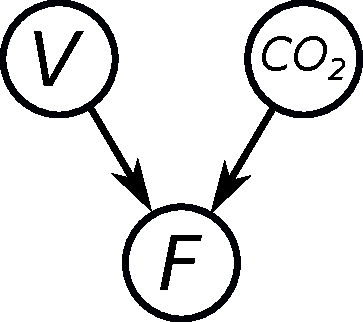
\includegraphics[width=1.2\textwidth]{fig/twoparents-3var.pdf}
%   \end{column}%
%   \begin{column}{0.8\textwidth}
%     \begin{itemize}
%      \item The container volume $V$.
%      \item The amount of $CO_2$.
%      \item The amount of time the fan is switched on $F$.
%     \end{itemize}
%   \end{column}
%  \end{columns}
%  \vspace{6mm}
%   $F$ depends on the amount of $CO_2$ and the volume $V$.
%   \[p(f,co_2,v) = \only<1>{\alert{\text{You've got 3 minutes.}}}\only<2>{p(f|co_2,v)\;p(co_2)\;p(v)}\]
% \end{frame}
% 
% %%%%%%%%%%%%%%%%%%%%%%%%%%%%%%%%%%%%%%%%%%%%%%%%%%%%%%%%%%%%%%
% \begin{frame}{3-variable models: cascaded}
% \begin{columns}
%   \begin{column}{0.12\textwidth}%
%    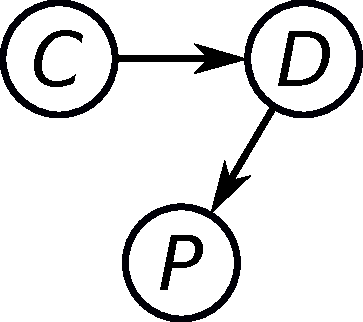
\includegraphics[width=1.2\textwidth]{fig/cascaded-3var.pdf}
%   \end{column}%
%   \begin{column}{0.8\textwidth}
%     \begin{itemize}
%      \item The amount of cider $C$.
%      \item How much you dance $D$.
%      \item The amount of pictures on facebook $P$ the day after.
%     \end{itemize}
%   \end{column}
%  \end{columns}
%  \vspace{6mm}
%   The amount of dance $D$ is clearly dependent on $C$, so is $P$ on $D$.
%   \[p(p,d,c) = \only<1>{\alert{\text{You've got 3 minute.}}}\only<2>{p(p|d)\;p(d|c)\;p(c)}\]
% \end{frame}
% 
% %%%%%%%%%%%%%%%%%%%%%%%%%%%%%%%%%%%%%%%%%%%%%%%%%%%%%%%%%%%%%%
% \begin{frame}{n-variable models}
%  One would like to end up studying models with many variables,\\ but first we need to understand the basics.
%  \begin{figure}
%  \centering
%  \only<1>{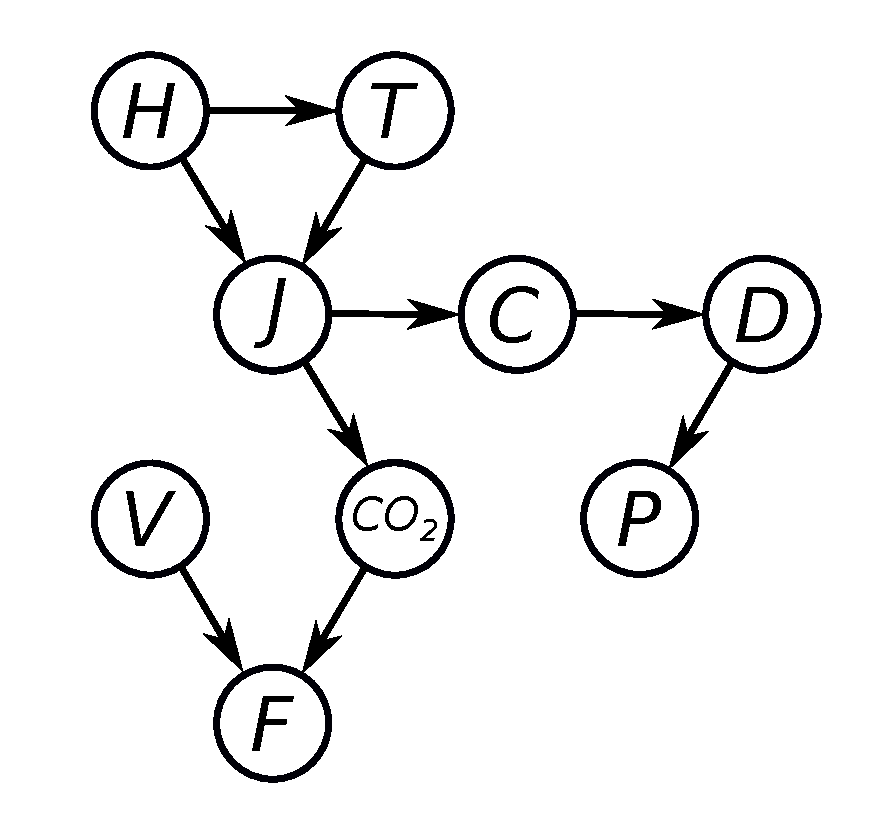
\includegraphics[width=0.4\textwidth]{fig/huge-muvar.pdf}}%
%  \only<2>{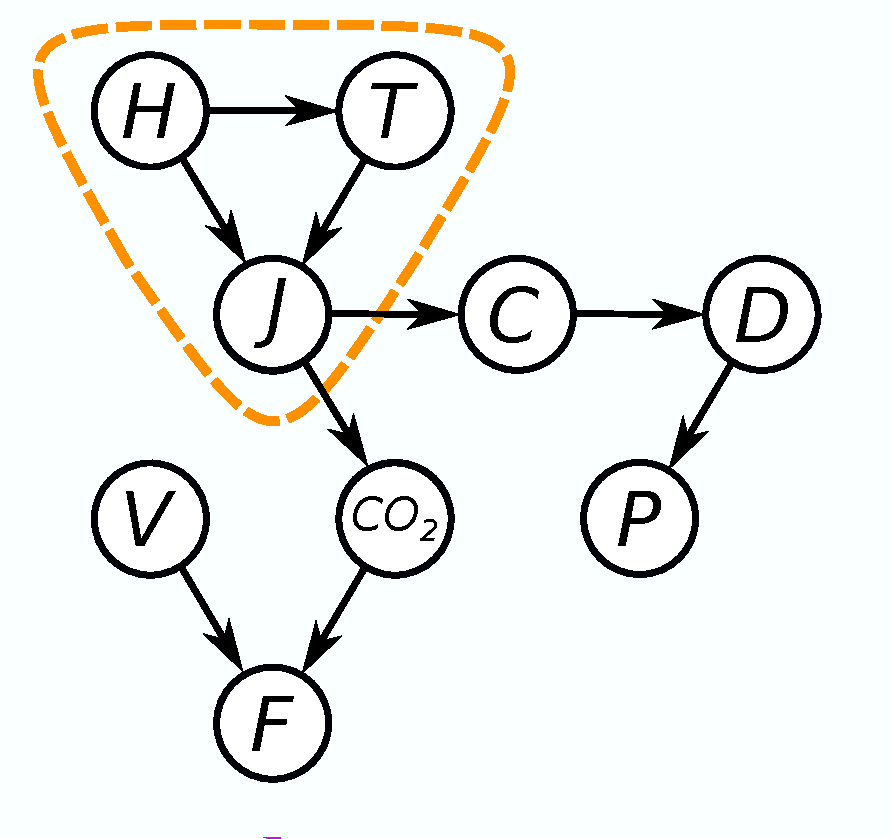
\includegraphics[width=0.4\textwidth]{fig/huge-muvar-full.pdf}}%
%  \only<3>{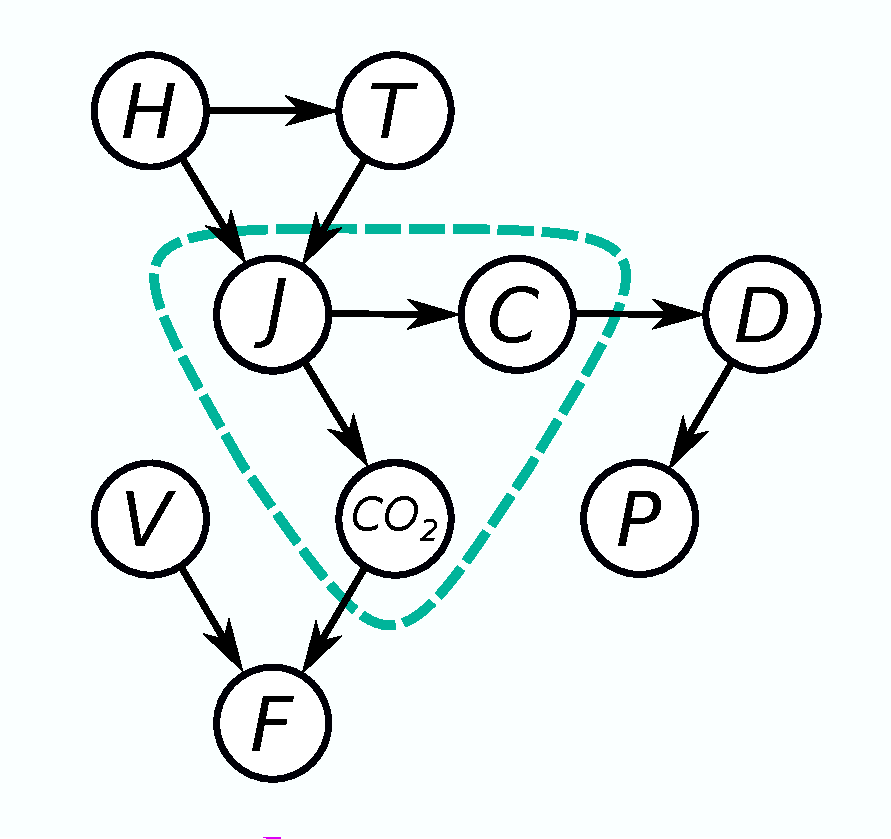
\includegraphics[width=0.4\textwidth]{fig/huge-muvar-twokids.pdf}}%
%  \only<4>{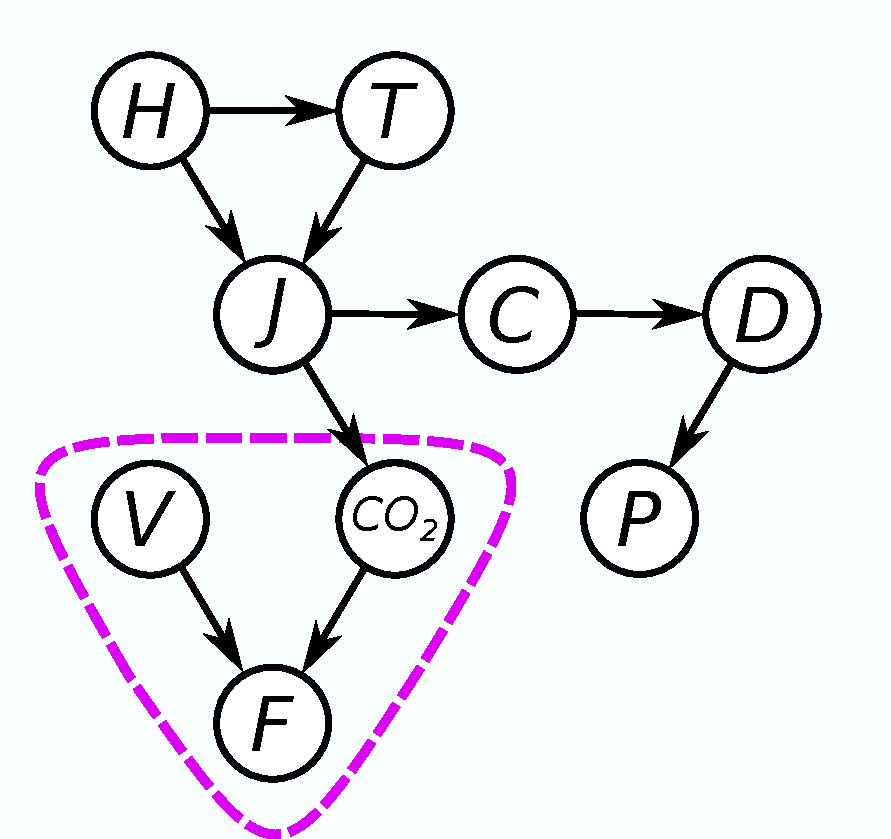
\includegraphics[width=0.4\textwidth]{fig/huge-muvar-twoparents.pdf}}%
%  \only<5>{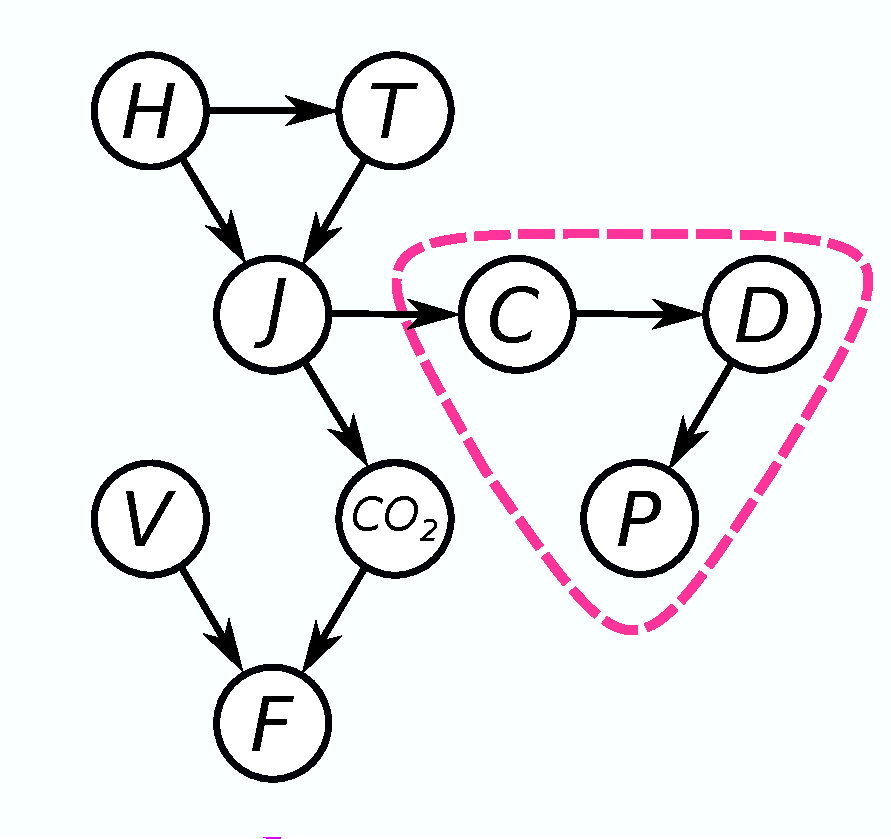
\includegraphics[width=0.4\textwidth]{fig/huge-muvar-cascaded.pdf}}%
%  \end{figure} 
%  \only<2->{Four minimals schemes: Full, }\only<3->{Two kids, }\only<4->{Two parents }\only<5>{and Cascaded.}
% \end{frame}

%%%%%%%%%%%%%%%%%%%%%%%%%%%%%%%%%%%%%%%%%%%%%%%%%%%%%%%%%%%%%%
\begin{frame}{3-variable models: taxonomy}
 \begin{columns}
  \begin{column}{0.12\textwidth}%
   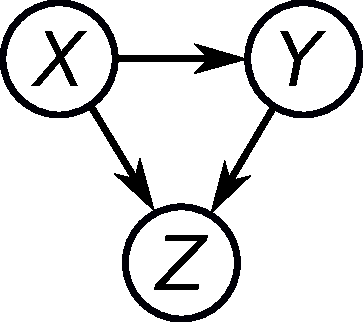
\includegraphics[width=1.2\textwidth]{fig/full-xyz.pdf}
  \end{column}%
  \begin{column}{0.8\textwidth}
  \textbf{Full}\;\; all dependencies are set:
  \[p(x,y,z) = p(z|x,y)p(y|x)p(x)\]
  \end{column}
 \end{columns}\vspace{3mm}
 \pause
  \begin{columns}
  \begin{column}{0.12\textwidth}%
   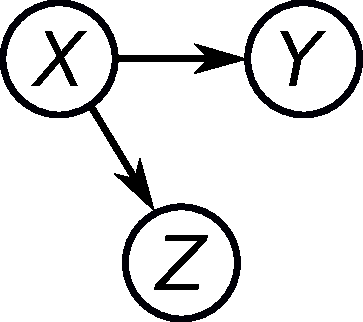
\includegraphics[width=1.2\textwidth]{fig/twokids-xyz.pdf}
  \end{column}%
  \begin{column}{0.8\textwidth}
  \textbf{Two-kids}\;\; $Y$-$Z$ dependency missing:
  \[p(x,y,z) = p(z|x{\color{lightgray},y})p(y|x)p(x)\]
  \end{column}
 \end{columns}\vspace{3mm}
 \pause
 \begin{columns}
  \begin{column}{0.12\textwidth}%
   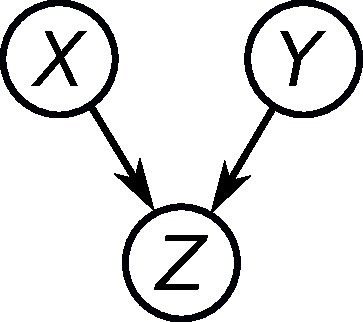
\includegraphics[width=1.2\textwidth]{fig/twoparents-xyz.pdf}
  \end{column}%
  \begin{column}{0.8\textwidth}
  \textbf{Two-parents}\;\; $X$-$Y$ dependency missing:
  \[p(x,y,z) = p(z|x,y)p(y{\color{lightgray}|x})p(x)\]
  \end{column}
 \end{columns}\vspace{3mm}
 \pause
 \begin{columns}
  \begin{column}{0.12\textwidth}%
   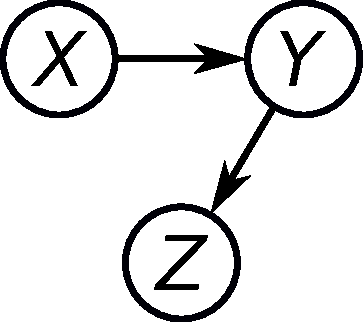
\includegraphics[width=1.2\textwidth]{fig/cascaded-xyz.pdf}
  \end{column}%
  \begin{column}{0.8\textwidth}
  \textbf{Cascaded}\;\; $X$-$Z$ dependency missing:
  \[p(x,y,z) = p(z|{\color{lightgray}x,}\ y)p(y|x)p(x)\]
  \end{column}
 \end{columns}
\end{frame}

% %%%%%%%%%%%%%%%%%%%%%%%%%%%%%%%%%%%%%%%%%%%%%%%%%%%%%%%%%%%%%%
% \begin{frame}{3-variable models: let's play! (I)}
%  \begin{columns}
%   \begin{column}{0.12\textwidth}%
%    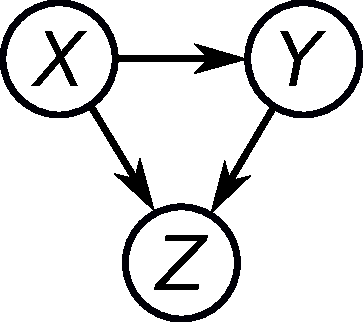
\includegraphics[width=1.2\textwidth]{fig/full-xyz.pdf}
%   \end{column}%
%   \begin{column}{0.8\textwidth}
%   \textbf{Full}\;\; all dependencies are set:
%   \[p(x,y,z) = p(z|x,y)p(y|x)p(x)\]
%   \end{column}
%  \end{columns}
%  \vspace{4mm}
%  Let's find $p(x,y|z)$ in terms of the model's distributions\\
%  (i.e.\ previous equation). \only<1>{\alert{You've got 5 minutes}\vspace{4mm}
%  
%  \underline{Hint}: use the joint probability.}\pause
%  \[p(x,y|z) = \frac{p(x,y,z)}{p(z)} \pause = \frac{p(z|x,y)p(y|x)p(x)}{\pause\int_{{\cal X}\times{\cal Y}}p(x',y',z)\textrm{d}x'\textrm{d}y'}\]
%  \pause with
%  \[ \int_{{\cal X}\times{\cal Y}}p(x',y',z)\textrm{d}x'\textrm{d}y' = \int_{{\cal X}\times{\cal Y}} p(z|x',y')p(y'|x')p(x') \textrm{d}x'\textrm{d}y'\]
% \end{frame}

%%%%%%%%%%%%%%%%%%%%%%%%%%%%%%%%%%%%%%%%%%%%%%%%%%%%%%%%%%%%%%
\begin{frame}{3-variable models: Two-kids}
 \begin{columns}
  \begin{column}{0.12\textwidth}%
   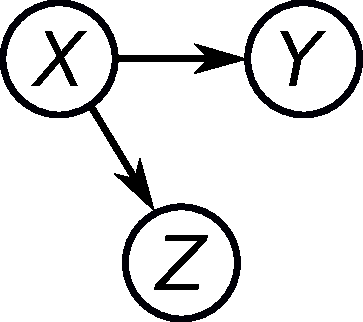
\includegraphics[width=1.2\textwidth]{fig/twokids-xyz.pdf}
  \end{column}%
  \begin{column}{0.8\textwidth}
  \textbf{Two-kids}\;\; $p(x,y,z) = p(z|x)p(y|x)p(x)$.
  \end{column}
 \end{columns}
 \vspace{4mm}
\exercise{two-kinds-independence}{Prove that in the Two-kids model:
\[
 p(y|z)\neq p(y) \qquad \text{and} \qquad  p(y|z,x) =  p(y|x)
\]
}\vspace{2mm}
\begin{itemize}
 \item The first statement is equivalent to say that $y$ and $z$ are not independent.
 \item The second statement, says that $y$ and $z$ are \textbf{conditionally independent} w.r.t.\ $x$.
\end{itemize}
\end{frame}

%%%%%%%%%%%%%%%%%%%%%%%%%%%%%%%%%%%%%%%%%%%%%%%%%%%%%%%%%%%%%%
\begin{frame}{3-variable models: Two-parents}
\begin{columns}
  \begin{column}{0.12\textwidth}%
   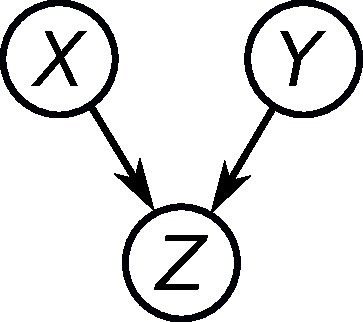
\includegraphics[width=1.2\textwidth]{fig/twoparents-xyz.pdf}
  \end{column}%
  \begin{column}{0.8\textwidth}
  \textbf{Two-parents}\;\; $p(x,y,z) = p(z|x,y)p(x)p(y)$.
  \end{column}
 \end{columns}
 \vspace{4mm}
\exercise{two-parents-independence}{Prove that in the Two-parents model:
\begin{equation}
 p(y|x) = p(x) \qquad \text{and} \qquad p(x|y,z) \neq p(x|z).
\end{equation}}\vspace{2mm}
We are in the opposite case:
\begin{itemize}
 \item The first statement says that $y$ and $x$ are independent.
 \item The second statement says that $y$ and $x$ are conditionally dependent w.r.t.\ $z$.
\end{itemize}
\end{frame}

% %%%%%%%%%%%%%%%%%%%%%%%%%%%%%%%%%%%%%%%%%%%%%%%%%%%%%%%%%%%%%%
% \begin{frame}{3-variable models: let's play! (IV)}
% \begin{columns}
%   \begin{column}{0.12\textwidth}%
%    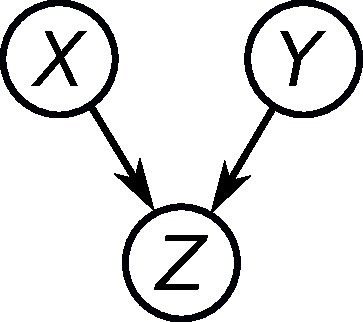
\includegraphics[width=1.2\textwidth]{fig/twoparents-xyz.pdf}
%   \end{column}%
%   \begin{column}{0.8\textwidth}
%   \textbf{Two-parents}\;\; $p(x,y,z) = p(z|x,y)p(x)p(y)$.
%   \end{column}
%  \end{columns}
%  \vspace{4mm}
%  Let's find $p(x,y|z)$ in terms of the model's distributions\\
%  (i.e.\ previous equation). \only<1>{\alert{You've got 5 minutes}\vspace{4mm}}\pause
%  \[ p(x,y|z)=\frac{p(x,y,z)}{p(z)}\pause = \frac{p(z|x,y)p(x)p(y)}{\int_{{\cal X}\times{\cal Y}}p(z|x',y')p(x')p(y')\textrm{d}x'\textrm{d}y'}. \]
%  \pause
%  We can also compute:
%  \[ p(x,y) = p(x)p(y).\]
%  $X$ and $Y$ are independent, but not conditionally independent given $Z$.
% \end{frame}

%%%%%%%%%%%%%%%%%%%%%%%%%%%%%%%%%%%%%%%%%%%%%%%%%%%%%%%%%%%%%%
\begin{frame}{3-variable models: Cascaded}
\begin{columns}
  \begin{column}{0.12\textwidth}%
   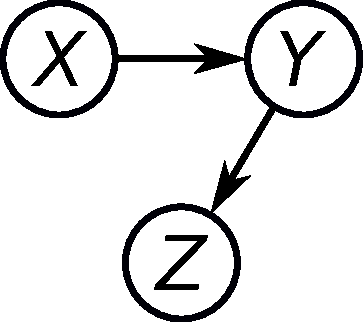
\includegraphics[width=1.2\textwidth]{fig/cascaded-xyz.pdf}
  \end{column}%
  \begin{column}{0.8\textwidth}
  \textbf{Cascaded}\;\; $p(x,y,z) = p(z|y)p(y|x)p(x)$.
  \end{column}
 \end{columns}
 \vspace{4mm}
    \exercise{cascaded-independence}{Prove that in the Cascaded model:
    \begin{equation}
    p(x,z)\neq p(x)p(z) \qquad\text{and}\qquad p(x,z|y) = p(x|y)p(z|y).
    \end{equation}
    }\vspace{2mm}

In this case, we obtain similar results than with the Two-kids model.\vspace{8mm}\pause

\remark{ind-vs-cond-ind}{At this point it should be clear that independence and conditional independence are \textbf{two very different properties} of random variables.}
\end{frame}

%%%%%%%%%%%%%%%%%%%%%%%%%%%%%%%%%%%%%%%%%%%%%%%%%%%%%%%%%%%%%%
\begin{frame}{Conditional Independence: Definition}
\remark{cond-ind-definition}{
Let $x$, $y$, and $z$ be random variables, we say that $x$ and $y$ are \textbf{conditionally independent} given $z$, and write $x\indep y \;|\; z$, iff one of the following equivalent expressions holds:
\begin{itemize}
 \item $p(x,y|z) = p(x|z)p(y|z)$
 \item $p(x|y,z) = p(x|z)$
 \item $p(y|x,z) = p(y|z)$
\end{itemize}
}\vspace{3mm}
\end{frame}
% 
% %%%%%%%%%%%%%%%%%%%%%%%%%%%%%%%%%%%%%%%%%%%%%%%%%%%%%%%%%%%%%%
% \begin{frame}{Conditional Independence: 3 Gaussian variables}
% Let $x$, $y$ and $z$ three random variables following:\vspace{3mm}
% \begin{columns}
%  \begin{column}{0.35\textwidth}
%  \vspace{-4mm}
% \begin{align*}
% x& = \mu_x+\nu_x\varepsilon_x,\\
% y& = \mu_y+\nu_y\varepsilon_y+px,\\
% z& = \mu_z+\nu_z\varepsilon_z+cx+ky,
% \end{align*} 
%  \end{column}with\hspace{8mm}%
%  \begin{column}{0.4\textwidth}
%   $\varepsilon_*,\sim{\cal N}(0,1)$,\\
%   $\mu_*\in\mathbb{R}$ and $\nu_*\in\mathbb{R}^+$\\
%   {\footnotesize ($*$ is $x$, $y$, or $z$.)}\\
%   $p,c,k\in\mathbb{R}$.
%  \end{column}
% \end{columns}\vspace{3mm}
% \pause
% Then, the joint probability $p(x,y,z)$ is a {\bf multivariate Gaussian}:
% \[p(x,y,z) = \frac{1}{\sqrt{|2\pi\Sigma|}}\exp\Big(-\frac{1}{2} (v-\mu)^\top\Sigma^{-1}(v-\mu) \Big),\]
% where $v=(x,y,z)^\top$ is the joint vector and $\Sigma$  and $\mu$ are the so-called {\bf covariance matrix} and {\bf mean vector}.\\
% ($\rightarrow$ check Bishop's book, section 2.3 until 2.3.4).\vspace{5mm}\\
% {\bf Homework}: (i) prove that you obtain such a Gaussian, (ii) compute $\mu$.
%  
% \end{frame}
% 
% 
% %%%%%%%%%%%%%%%%%%%%%%%%%%%%%%%%%%%%%%%%%%%%%%%%%%%%%%%%%%%%%%
% 
% \begin{frame}{Conditional Independence: 3 Gaussian variables (II)}
%  $\Sigma$ in the previous equation takes the following form:
% \[\Sigma^{-1} = \left(\begin{array}{ccc}
% \frac{1}{\nu_x}+\frac{p^2}{\nu_y}+\frac{c^2}{\nu_z} & \frac{p}{\nu_y} & \frac{c}{\nu_z} \\
% \frac{p}{\nu_y} & \frac{1}{\nu_y}+\frac{k^2}{\nu_z} & \frac{k}{\nu_z} \\
% \frac{c}{\nu_z} & \frac{k}{\nu_z} & \frac{1}{\nu_z}
% \end{array}\right)\]\\
% \pause
% \noindent For which values of $p,k,c$ you obtain the models:\\ two-parents, two-kids and cascaded ? \alert{You've got 5 minutes}.\vspace{3mm}\\
% \begin{center}
%   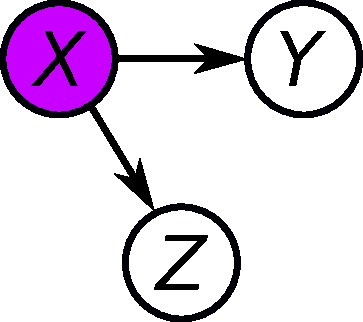
\includegraphics[width=0.15\textwidth]{fig/twokids-xyz-color.pdf}\hspace{4mm}%
%   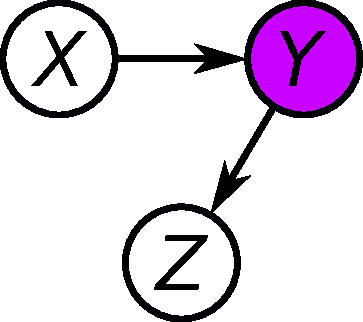
\includegraphics[width=0.15\textwidth]{fig/cascaded-xyz-color.pdf}\hspace{4mm}%
%   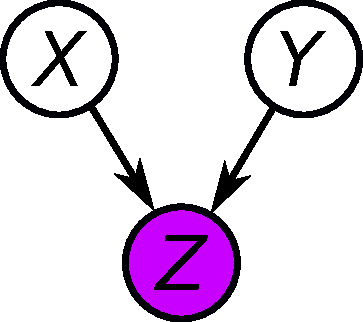
\includegraphics[width=0.15\textwidth]{fig/twoparents-xyz-color.pdf}\\
% \end{center}
% {\bf Homework}: prove the expression for $\Sigma$.
% \end{frame}

\subsection{D-separation}

%%%%%%%%%%%%%%%%%%%%%%%%%%%%%%%%%%%%%%%%%%%%%%%%%%%%%%%%%%%%%%

\begin{frame}{Motivation}
Let's consider the following variables and dependencies.
\begin{center}
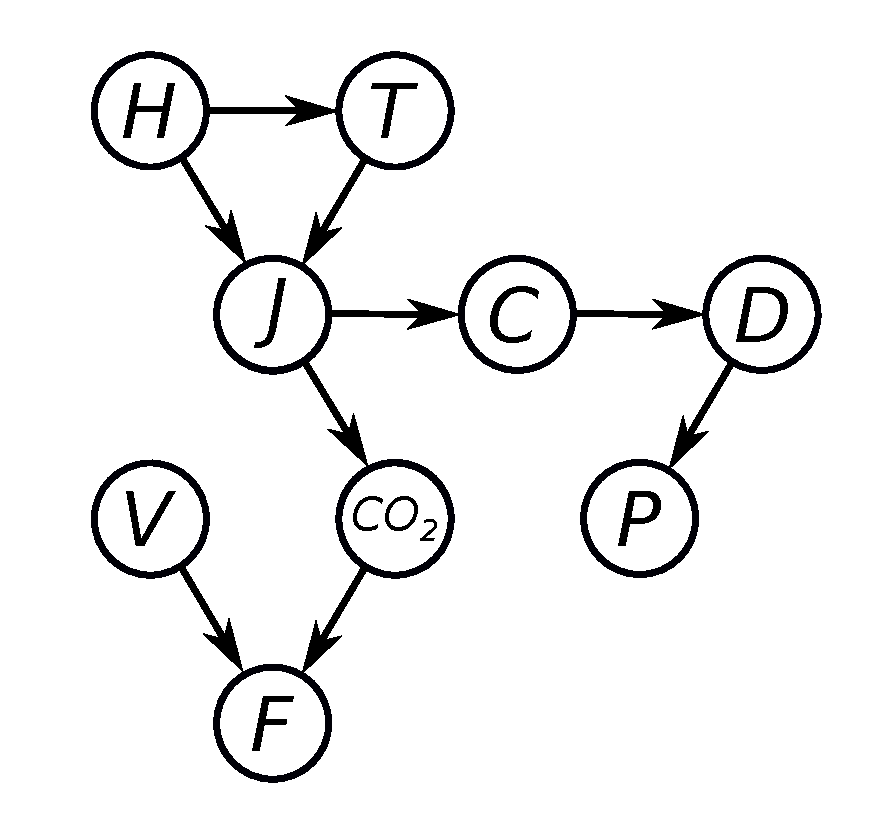
\includegraphics[width=0.4\textwidth]{fig/huge-muvar.pdf}
\end{center}
Is $P \indep V \;|\; T$ ? How would you do it ? Is the previous strategy scalable ?
\end{frame}

%%%%%%%%%%%%%%%%%%%%%%%%%%%%%%%%%%%%%%%%%%%%%%%%%%%%%%%%%%%%%%

\begin{frame}{Basics}
 Let us recall the 3-var models:\vspace{3mm}\\
 \begin{columns}
  \begin{column}{0.12\textwidth}%
   \only<1->{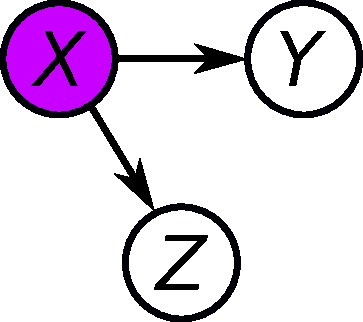
\includegraphics[width=1.2\textwidth]{fig/twokids-xyz-color.pdf}\vspace{4mm}\\}
   \only<2->{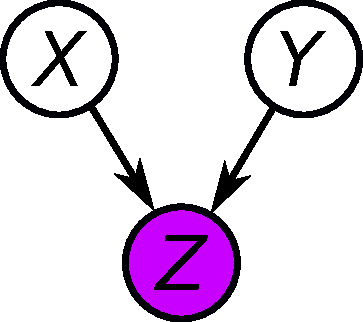
\includegraphics[width=1.2\textwidth]{fig/twoparents-xyz-color.pdf}\vspace{4mm}\\}
   \only<3->{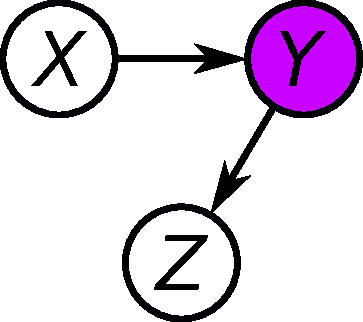
\includegraphics[width=1.2\textwidth]{fig/cascaded-xyz-color.pdf}}
  \end{column}%
  \begin{column}{0.85\textwidth}
  \only<1->{\textbf{Two kids}\;\; The path from $Z$ to $Y$ is called ``tail-to-tail.''
    \[p(z,y|{\color{mypurple}x}) = p(z|{\color{mypurple}x})p(y|{\color{mypurple}x}) \] \vspace{-2mm}\\}
  
  \only<2->{\textbf{Two parents}\;\; The path from $X$ to $Y$ is called ``head-to-head.''
  \[p(x,y|{\color{mypurple}z}) \neq p(x|{\color{mypurple}z})p(y|{\color{mypurple}z})\] \vspace{-2mm}\\}
  
  \only<3->{\textbf{Cascaded}\;\; The path from $X$ to $Z$ is called ``head-to-tail.''
  \[p(x,z|{\color{mypurple}y}) = p(x|{\color{mypurple}y})p(z|{\color{mypurple}y})\]} 
  \end{column}
 \end{columns}%\vspace{4mm}
%  \only<4->{\alert{Please check Section 8.2 of Bishop's book.}}
\end{frame}

%%%%%%%%%%%%%%%%%%%%%%%%%%%%%%%%%%%%%%%%%%%%%%%%%%%%%%%%%%%%%%

\begin{frame}{Path blocking}
\begin{center}
  \hspace{3mm}{\bf Two-kids}\hspace{6mm}{\bf Cascaded}\hspace{16mm}{\bf Two-parents}\vspace{1mm}\\
  \hspace{3mm}{\small tail-to-tail}\hspace{6mm}{\small head-to-tail}\hspace{18mm}{\small head-to-head}\vspace{2mm}\\
  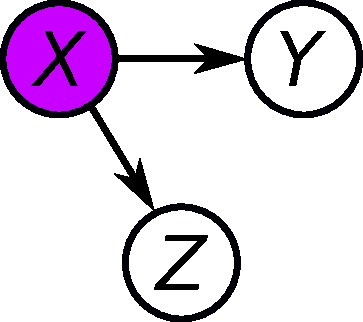
\includegraphics[width=0.15\textwidth]{fig/twokids-xyz-color.pdf}\hspace{4mm}%
  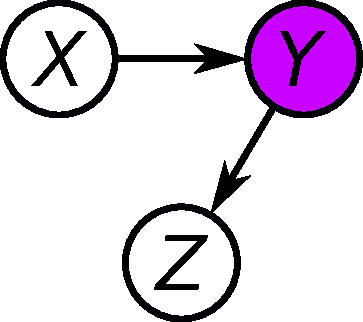
\includegraphics[width=0.15\textwidth]{fig/cascaded-xyz-color.pdf}\hspace{16mm}%
  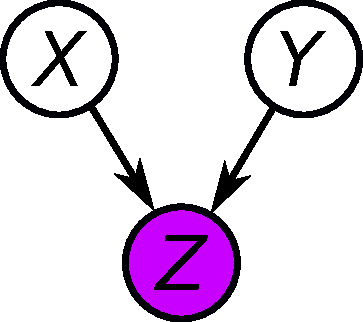
\includegraphics[width=0.15\textwidth]{fig/twoparents-xyz-color.pdf}\\
\end{center}
\pause
 {The purple node {\bf ``blocks'' the path} in two-kids/tail-to-tail \& cascaded/head-to-tail $\rightarrow$ conditional independence.\vspace{7mm}\\
 \pause
 The purple node {\bf ``unblocks'' the path} in two-parents/head-to-head $\rightarrow$ conditional dependence.\\}
 \pause
 In the two-parents, $Z$ or any descendant of $Z$ will unblock the path.
\end{frame}

% %%%%%%%%%%%%%%%%%%%%%%%%%%%%%%%%%%%%%%%%%%%%%%%%%%%%%%%%%%%%%%
% 
% \begin{frame}{D-separation: 6-dimensional Gaussian}
%  \textbf{[1D]} \hspace{3mm}Let $X$, $Y$ and $Z$ three random variables following:\vspace{3mm}
% \begin{columns}
%  \begin{column}{0.1\textwidth}
%   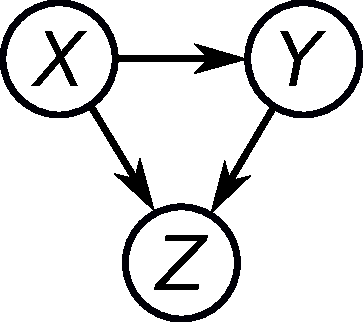
\includegraphics[width=1.5\textwidth]{fig/full-xyz.pdf}
%  \end{column}
% \begin{column}{0.3\textwidth}
%  \vspace{-4mm}
% \begin{align*}
% X& = \varepsilon_x,\\
% Y& = \varepsilon_y+pX,\\
% Z& = \varepsilon_z+cX+kY,
% \end{align*}  
%  \end{column}with\hspace{8mm}%
%  \begin{column}{0.25\textwidth}
%   $\epsilon_*,\sim{\cal N}(\mu_*,\nu_*)$,\\
%   
%   $p,c,k\in\mathbb{R}$.
%  \end{column}
% \end{columns}\vspace{3mm}
% \pause
%  \textbf{[2D]} \hspace{3mm}Let $X$, $Y$ and $Z$ three random \textcolor{green}{vectors} following:\vspace{3mm}
% \begin{columns}
%  \begin{column}{0.1\textwidth}
%   \only<2>{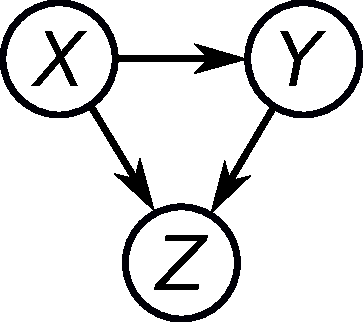
\includegraphics[width=1.5\textwidth]{fig/full-xyz.pdf}}%
%   \only<3->{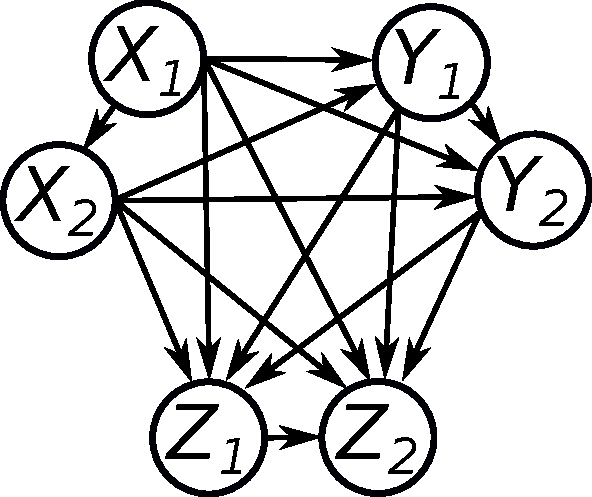
\includegraphics[width=1.5\textwidth]{fig/full-multivar.pdf}}%
%  \end{column}
% \begin{column}{0.3\textwidth}
%  \vspace{-4mm}
% \begin{align*}
% X& = \varepsilon_x,\\
% Y& = \varepsilon_y+PX,\\
% Z& = \varepsilon_z+CX+KY,
% \end{align*}  
%  \end{column}with\hspace{8mm}%
%  \begin{column}{0.25\textwidth}
%   $\epsilon_*,\sim{\cal N}({\color{green}M_*},{\color{green}N_*})$,\\
%   
%   $P,C,K\in\mathbb{R}^{\color{green}2\times 2}$.\\
%   
%   \only<3->{$X=({\color{green}X_1},{\color{green}X_2})^\top$ {\footnotesize(same for $Y$ and $Z$)}.}
%  \end{column}
% \end{columns}\vspace{3mm}
% \pause
% In this case, $\color{green}M_*\in\mathbb{R}^2$ and $\color{green}N_*\in\mathbb{R}^{2\times 2}$.\\ Each $\epsilon_*$ is a {\bf multivariate Gaussian}.\\
% $V=(X^\top,Y^\top,Z^\top)^\top$ is also a multivariate Gaussian.
% \end{frame}

% %%%%%%%%%%%%%%%%%%%%%%%%%%%%%%%%%%%%%%%%%%%%%%%%%%%%%%%%%%%%%%
% 
% \begin{frame}{D-separation: 6-dimensional Gaussian (II)}
%  \begin{columns}
%  \begin{column}{0.1\textwidth}
%    \only<1-2>{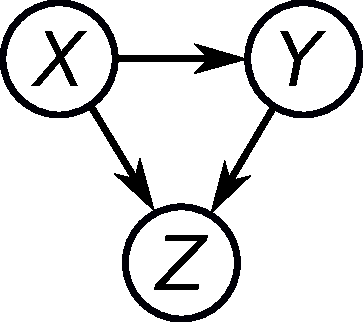
\includegraphics[width=1.5\textwidth]{fig/full-xyz.pdf}}%
%    \only<3>{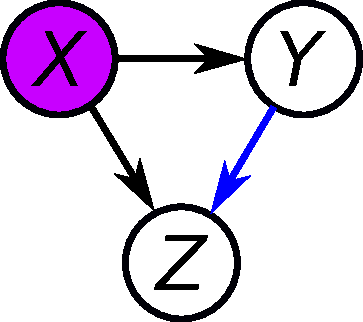
\includegraphics[width=1.5\textwidth]{fig/twokids-xyz-blue.pdf}}%
%    \only<4>{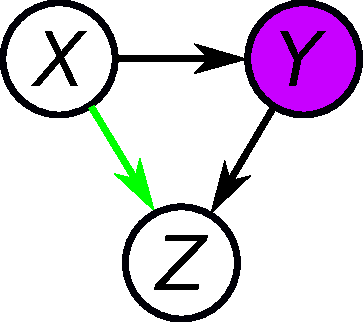
\includegraphics[width=1.5\textwidth]{fig/cascaded-xyz-green.pdf}}%
%    \only<5>{\includegraphics[width=1.5\textwidth]{fig/twoparents-xyz-red.pdf}}%
%    \only<6>{\includegraphics[width=1.5\textwidth]{fig/full-xyz-colorful.pdf}}%
%  \end{column}
% \begin{column}{0.3\textwidth}
%  \vspace{-4mm}
% \begin{align*}
% X& = \varepsilon_x,\\
% Y& = \varepsilon_y+{\only<5,6>{\color{red}}pX},\\
% Z& = \varepsilon_z+{\only<4,6>{\color{green}}cX}+{\only<3,6>{\color{blue}}kY},
% \end{align*}  
% \end{column}
%  \begin{column}{0.1\textwidth}
%    \only<1-2>{\includegraphics[width=1.5\textwidth]{fig/full-multivar.pdf}}%
%    \only<3>{\includegraphics[width=1.5\textwidth]{fig/full-multivar-twokids-blue.pdf}}%
%    \only<4>{\includegraphics[width=1.5\textwidth]{fig/full-multivar-cascaded-green.pdf}}%
%    \only<5>{\includegraphics[width=1.5\textwidth]{fig/full-multivar-twoparents-red.pdf}}%
%    \only<6>{\includegraphics[width=1.5\textwidth]{fig/full-multivar-colorful.pdf}}%
%  \end{column}
% \begin{column}{0.3\textwidth}
%  \vspace{-4mm}
% \begin{align*}
% X& = \varepsilon_x,\\
% Y& = \varepsilon_y+{\only<5,6>{\color{red}}PX},\\
% Z& = \varepsilon_z+{\only<4,6>{\color{green}}CX}+{\only<3,6>{\color{blue}}KY},
% \end{align*}  
%  \end{column}
% \end{columns}\vspace{3mm}\pause
% The covariance matrix $\Sigma$ in the 2D-case writes (check Bishop's book):
%   \[\Sigma^{-1} = \left(\begin{array}{ccc}
%   N_x^{-1} + {\only<5,6>{\color{red}}P^\top N_y^{-1}P} + {\only<4,6>{\color{green}}C^\top N_z^{-1}C} & {\only<5,6>{\color{red}}N_y^{-1}P} & 
% {\only<4,6>{\color{green}}N_z^{-1}C} \\
%   {\only<5,6>{\color{red}}P^\top N_y^{-1}} & N_y^{-1} + {\only<3,6>{\color{blue}}K^\top N_z^{-1} K} & {\only<3,6>{\color{blue}}N_z^{-1}K} \\
%   {\only<4,6>{\color{green}}C^\top N_z^{-1}} & {\only<3,6>{\color{blue}}K^\top N_z^{-1}} & N_z^{-1}
% \end{array}\right)\]
% 
% \only<3->{{\only<3,6>{\color{blue}}{\bf Two-kids}} (tail-to-tail): $p(y,z|{\only<3>{\color{mypurple}}x}) = 
% p(y|{\only<3>{\color{mypurple}}x})p(z|{\only<3>{\color{mypurple}}x})$}\vspace{1mm}
% 
% \only<4->{{\only<4,6>{\color{green}}{\bf Cascaded}} (head-to-tail): $p(x,z|{\only<4>{\color{mypurple}}y}) = 
% p(x|{\only<4>{\color{mypurple}}y})p(z|{\only<4>{\color{mypurple}}y})$}\vspace{1mm}
% 
% \only<5->{{\only<5,6>{\color{red}}{\bf Two-parents}} (head-to-head): $p(x,y|{\only<5>{\color{mypurple}}z}) \neq 
% p(x|{\only<5>{\color{mypurple}}z})p(y|{\only<5>{\color{mypurple}}z})$}\vspace{1mm}
% 
% \only<6>{\begin{block}{}
% \centering
% This gives us hope for more complicated models!
% \end{block}}
% 
% \end{frame}

%%%%%%%%%%%%%%%%%%%%%%%%%%%%%%%%%%%%%%%%%%%%%%%%%%%%%%%%%%%%%%

\begin{frame}{Path blocking (revisited)}

{\small (Let me change the variable names)}
\begin{center}
  \hspace{3mm}{\bf Two-kids}\hspace{6mm}{\bf Cascaded}\hspace{16mm}{\bf Two-parents}\vspace{1mm}\\
  \hspace{3mm}{\small tail-to-tail}\hspace{6mm}{\small head-to-tail}\hspace{18mm}{\small head-to-head}\vspace{2mm}\\
  \includegraphics[width=0.15\textwidth]{fig/twokids-abc-color.pdf}\hspace{4mm}%
  \includegraphics[width=0.15\textwidth]{fig/cascaded-abc-color.pdf}\hspace{16mm}%
  \includegraphics[width=0.15\textwidth]{fig/twoparents-abc-color.pdf}\\
\end{center}
\only<2->{Tail-to-tail \& head-to-tail $\rightarrow A \indep B \,|\, C$.\vspace{3mm}\\}
\only<3->{Head-to-head $\rightarrow A \not\indep B \,|\, C$ or any descendant of $C$.\vspace{5mm}\\}
\only<4->{$\Rightarrow$ If $A \indep B \,|\, C$, nodes within tail-to-tail or head-to-tail can be in $C$ and nodes within head-to-head or any of their descendents must not be in $C$.}
\end{frame}

%%%%%%%%%%%%%%%%%%%%%%%%%%%%%%%%%%%%%%%%%%%%%%%%%%%%%%%%%%%%%%

\begin{frame}{Path blocking (definition)}
\remark{blocked-path}{\small Let $A$, $B$ and $C$ be three non-intersecting sets of nodes of a directed acyclic graph. A path from $A$ to $B$ is said to be blocked by $C$ if it includes a node that either:
\begin{itemize}
\item the path meets tail-to-tail or head-to-tail at the node and the node is in C;
\item the path meets head-to-head at the node and neither the node nor any of its descendants are in C.
\end{itemize}}\vspace{3mm}\pause
  \begin{columns}
   \begin{column}{0.25\textwidth}
    \only<1,6>{\includegraphics[width=\textwidth]{fig/blockedpaths.pdf}}%
    \only<2>{\includegraphics[width=\textwidth]{fig/blockedpaths-1.pdf}}%
    \only<3>{\includegraphics[width=\textwidth]{fig/blockedpaths-2.pdf}}%
    \only<4>{\includegraphics[width=\textwidth]{fig/blockedpaths-3.pdf}}%
    \only<5>{\includegraphics[width=\textwidth]{fig/blockedpaths-4.pdf}}%
   \end{column}\hspace{2mm}
   \begin{column}{0.75\textwidth}
    {\small (Corresponds to Exercise: \ref{notes-ex:path-blocking}.)}
    \begin{itemize}
     \item<2-> Is {\only<2>{\color{green}}the path from $\{x\}$ to $\{v\}$} blocked by {\only<2>{\color{mypurple}}$\{u\}$}? \only<3->{Yes}
     \item<3-> Is {\only<3>{\color{green}}the path from $\{x\}$ to $\{v\}$} blocked by {\only<3>{\color{mypurple}}$\{y\}$}? \only<4->{No}
     \item<4-> Is {\only<4>{\color{green}}the path from $\{x\}$ to $\{v\}$} blocked by {\only<4>{\color{mypurple}}$\{z\}$}? \only<5->{No}
     \item<5-> Is {\only<5>{\color{green}}the path from $\{y\}$ to $\{v\}$} blocked by {\only<5>{\color{mypurple}}$\{u\}$}? \only<6->{Yes}
    \end{itemize}
   \end{column}
  \end{columns} 
\end{frame}

%%%%%%%%%%%%%%%%%%%%%%%%%%%%%%%%%%%%%%%%%%%%%%%%%%%%%%%%%%%%%%

\begin{frame}{D-separation}
\remark{d-separation}{Let $A$, $B$ and $C$ be three non-intersecting sets of nodes of a directed acyclic graph. $A$ and $B$ are \textbf{D-separated} by $C$, if all paths from any node from $A$ to $B$ are blocked by $C$.}\vspace{3mm}\pause

   \begin{columns}
   \begin{column}{0.25\textwidth}
    \only<1,5>{\includegraphics[width=\textwidth]{fig/blockedpaths.pdf}}%
    \only<2>{\includegraphics[width=\textwidth]{fig/D-separated-1.pdf}}%
    \only<3>{\includegraphics[width=\textwidth]{fig/D-separated-2.pdf}}%
    \only<4>{\includegraphics[width=\textwidth]{fig/D-separated-3.pdf}}%
    \end{column}\hspace{2mm}
   \begin{column}{0.7\textwidth}
   {\small (Corresponds to Exercise: \ref{notes-ex:d-separation}.)}
    \begin{itemize}
     \item<2-> Is {\only<2>{\color{green}}$\{X\}$} D-separated from {\only<2>{\color{cyan}}$\{V\}$} by {\only<2>{\color{mypurple}}$\{U\}$}? \only<3->{Yes}
     \item<3-> Is {\only<3>{\color{green}}$\{X\}$} D-separated from {\only<3>{\color{cyan}}$\{V\}$} by {\only<3>{\color{mypurple}}$\{Y\}$}? \only<4->{No}
     \item<4-> Is {\only<4>{\color{green}}$\{X\}$} D-separated from {\only<4>{\color{cyan}}$\{V\}$} by {\only<4>{\color{mypurple}}$\{Y,U\}$}? \only<5->{Yes}
    \end{itemize}

   \end{column}
  \end{columns}\vspace{3mm}
  \remark{dsep-cind}{$A$ and $B$ are D-separated by $C$ if and only if $A \indep B | C$.}
\end{frame}

%%%%%%%%%%%%%%%%%%%%%%%%%%%%%%%%%%%%%%%%%%%%%%%%%%%%%%%%%%%%%%

\subsection{Markovian dependencies}

%%%%%%%%%%%%%%%%%%%%%%%%%%%%%%%%%%%%%%%%%%%%%%%%%%%%%%%%%%%%%%

\begin{frame}{Markov models: introduction}
 Principle: each variable depends \textbf{only} on its closer neighbours. Examples:\vspace{5mm}\\
 \begin{columns}
  \begin{column}{0.4\textwidth}
    \includegraphics[width=\textwidth]{fig/temporal-simple.pdf}\vspace{5mm}\\%
    \only<2->{\includegraphics[width=\textwidth]{fig/temporal-hmm.pdf}\vspace{3mm}\\}%
    {\small Markov chain\only<2->{ (top)}.}\\
    \only<2->{\small Hidden Markov chain (bottom).}
  \end{column}
  \begin{column}{0.4\textwidth}
   \only<3->{\includegraphics[width=\textwidth]{fig/temporal2layer.pdf}\vspace{3mm} {\small Double hidden Markov chain.}}% 
  \end{column}
 \end{columns}
\end{frame}

\begin{frame}{D-separation in Markov models}
With the following model:
\begin{center}
\only<1,5>{\includegraphics[width=0.4\textwidth]{fig/temporal-hmm.pdf}}%
\only<2>{\includegraphics[width=0.4\textwidth]{fig/temporal-hmm-xt.pdf}}%
\only<3>{\includegraphics[width=0.4\textwidth]{fig/temporal-hmm-yt.pdf}}%
\only<4>{\includegraphics[width=0.4\textwidth]{fig/temporal-hmm-xtyt.pdf}}%
\end{center}
Is $\{X_{t-1}\}$ D-separated from $\{Y_{t+1}\}$ by ...\vspace{3mm}\\
\begin{itemize}
 \item<2-> {\only<2>{\color{mypurple}} $\{X_t\}$}? \only<2>{[1 minute]}\only<3->{Yes}
 \item<3-> {\only<3>{\color{mypurple}} $\{Y_t\}$}? \only<3>{[1 minute]}\only<4->{No}
 \item<4-> {\only<4>{\color{mypurple}} $\{X_t,Y_t\}$}? \only<4>{[1 minute]}\only<5->{Yes}
\end{itemize}
\end{frame}

\begin{frame}{D-separation in Markov models (II)}
With the following model:
\begin{center}
\only<1,5>{\includegraphics[width=0.4\textwidth]{fig/temporal-omm.pdf}}%
\only<2>{\includegraphics[width=0.4\textwidth]{fig/temporal-omm-xt.pdf}}%
\only<3>{\includegraphics[width=0.4\textwidth]{fig/temporal-omm-yt.pdf}}%
\only<4>{\includegraphics[width=0.4\textwidth]{fig/temporal-omm-xtyt.pdf}}%
\end{center}
Is $\{X_{t-1}\}$ D-separated from $\{Y_{t+1}\}$ by ...\vspace{3mm}\\
\begin{itemize}
 \item<2-> {\only<2>{\color{mypurple}} $\{X_t\}$}? \only<2>{[1 minute]}\only<3->{No}
 \item<3-> {\only<3>{\color{mypurple}} $\{Y_t\}$}? \only<3>{[1 minute]}\only<4->{Yes}
 \item<4-> {\only<4>{\color{mypurple}} $\{X_t,Y_t\}$}? \only<4>{[1 minute]}\only<5->{Yes}
\end{itemize}
\end{frame}

\begin{frame}{D-separation in Markov models (III)}
With the following model:
\begin{center}
\only<1,5>{\includegraphics[width=0.4\textwidth]{fig/temporal-ohmm.pdf}}%
\only<2>{\includegraphics[width=0.4\textwidth]{fig/temporal-ohmm-xt.pdf}}%
\only<3>{\includegraphics[width=0.4\textwidth]{fig/temporal-ohmm-yt.pdf}}%
\only<4>{\includegraphics[width=0.4\textwidth]{fig/temporal-ohmm-xtyt.pdf}}%
\end{center}
Is $\{X_{t-1}\}$ D-separated from $\{Y_{t+1}\}$ by ...\vspace{3mm}\\
\begin{itemize}
 \item<2-> {\only<2>{\color{mypurple}} $\{X_t\}$}? \only<2>{[1 minute]}\only<3->{No}
 \item<3-> {\only<3>{\color{mypurple}} $\{Y_t\}$}? \only<3>{[1 minute]}\only<4->{No}
 \item<4-> {\only<4>{\color{mypurple}} $\{X_t,Y_t\}$}? \only<4>{[1 minute]}\only<5->{Yes}
\end{itemize}
\end{frame}

\begin{frame}{D-separation in Markov models: summary}
Is $\{X_{t-1}\}$ D-separated from $\{Y_{t+1}\}$ by (left column) in (top row)?\vspace{5mm}
\begin{columns}
 \begin{column}{1cm}
 $ $\vspace{1.8cm}\\
 $\{X_t\}$\vspace{.5cm}\\
 $\{Y_t\}$\vspace{.5cm}\\
 $\{X_t,Y_t\}$
 \end{column}
 \begin{column}{0.25\textwidth}
 \centering
  \includegraphics[width=\textwidth]{fig/temporal-hmm.pdf}\vspace{3mm}\\
  Yes\vspace{.5cm}\\
  No\vspace{.5cm}\\
  Yes
 \end{column}\hspace{3mm}
  \begin{column}{0.25\textwidth}
 \centering
  \includegraphics[width=\textwidth]{fig/temporal-omm.pdf}\vspace{3mm}\\
  No\vspace{.5cm}\\
  Yes\vspace{.5cm}\\
  Yes
 \end{column}\hspace{3mm}
  \begin{column}{0.25\textwidth}
 \centering
  \includegraphics[width=\textwidth]{fig/temporal-ohmm.pdf}\vspace{3mm}\\
  No\vspace{.5cm}\\
  No\vspace{.5cm}\\
  Yes
 \end{column}
\end{columns}\vspace{8mm}
(\small Corresponds to Exercise~\ref{notes-ex:d-separation-mm}.)
\end{frame}

% \begin{frame}{More complex models}
% Let's play a little bit with these two models:
%  \begin{center}
%   \includegraphics[width=0.3\textwidth]{fig/temporal2layer.pdf}\hspace{5mm}
%   \includegraphics[width=0.35\textwidth]{fig/D-separation.pdf}
%  \end{center}
%  Find one example of D-separation and one example of non D-separation (in whatever case). [You've got 5 minutes]
% 
% \end{frame}

% \subsection{Markov Blanket (or Boundary)}

\begin{frame}{Markov blanket (or boundary)}
 Model example:
 \begin{center}
    \only<1>{\includegraphics[width=0.4\textwidth]{fig/D-separation.pdf}}%
    \only<2>{\includegraphics[width=0.4\textwidth]{fig/D-separation-K.pdf}}%
    \only<3>{\includegraphics[width=0.4\textwidth]{fig/D-separation-KBK.pdf}}%
    \only<4>{\includegraphics[width=0.4\textwidth]{fig/D-separation-L.pdf}}%
    \only<5>{\includegraphics[width=0.4\textwidth]{fig/D-separation-LBL.pdf}}%
    \only<6>{\includegraphics[width=0.4\textwidth]{fig/D-separation-C.pdf}}%
    \only<7>{\includegraphics[width=0.4\textwidth]{fig/D-separation-CBC.pdf}}%
    \only<8>{\includegraphics[width=0.4\textwidth]{fig/D-separation-E.pdf}}%
    \only<9>{\includegraphics[width=0.4\textwidth]{fig/D-separation-EBE.pdf}}%
 \end{center}
 \pause
 For a given node $K$, what is the minimal set of variables ${\cal B}_K$ so that:
  \[p(K|\text{all except }K) = p(K|{\cal B}_K)\text{?}\qquad \only<3->{{\cal B}_K=\{G\}}\]
  \only<4->{For $L$?} \only<5->{$\quad{\cal B}_L=\{F,G,H\}$ because $F,G,H$ are {\bf parents} of $L$.\\}
  \only<6->{For $C$?} \only<7->{$\quad{\cal B}_C=\{B,D,F\}$ because $B$ ($F,D$) is parent ({\bf children}) of $C$.\\}
  \only<8->{For $E$?} \only<9->{$\quad{\cal B}_E=\{A,B,I,J\}$ because $A,B$ ($I$) are parents (children) of $E$ and $J$ is {\bf co-parent} of $E$.\\}
  \only<2,4,6,8>{You've got 3 minutes!}
\end{frame}

\begin{frame}{Markov blanket: definition}
 \remark{markov-blanket-def}{The \textbf{Markov blanket} is the minimal set that D-separates a set of nodes from the rest of the graph.}
 \begin{center}
    {\includegraphics[width=0.3\textwidth]{fig/D-separation-LBL.pdf}}\hspace{4mm}%
    {\includegraphics[width=0.3\textwidth]{fig/D-separation-CBC.pdf}}\hspace{4mm}%
    {\includegraphics[width=0.3\textwidth]{fig/D-separation-EBE.pdf}}%  
 \end{center}
 \remark{markov-blanket-cons}{Construction of the Markov blanket.    Given a directed acyclic graph, and a node $x$ on that graph, the Markov blanket of $x$, ${\cal B}_x$ is the set of all parents, children and co-parents of $x$.}
\end{frame}


% \begin{frame}{Markov blanket: extra-example}
%  \ {\bf Aim}: Isolate $F$ from as many nodes as possible with blocked paths.\vspace{3mm}
%  \begin{center}
%   \only<1>{\includegraphics[width=0.4\textwidth]{fig/D-separation-F.pdf}}%
%   \only<2>{\includegraphics[width=0.4\textwidth]{fig/D-separation-F-C.pdf}}%
%   \only<3>{\includegraphics[width=0.4\textwidth]{fig/D-separation-F-C1.pdf}}%
%   \only<4>{\includegraphics[width=0.4\textwidth]{fig/D-separation-F-C2.pdf}}%
%   \only<5>{\includegraphics[width=0.4\textwidth]{fig/D-separation-F-CJ.pdf}}%
%   \only<6>{\includegraphics[width=0.4\textwidth]{fig/D-separation-F-CJ1.pdf}}%
%   \only<7>{\includegraphics[width=0.4\textwidth]{fig/D-separation-F-CJ2.pdf}}%
%   \only<8>{\includegraphics[width=0.4\textwidth]{fig/D-separation-F-CJB.pdf}}%
%   \only<9>{\includegraphics[width=0.4\textwidth]{fig/D-separation-F-CJB1.pdf}}%
%   \only<10>{\includegraphics[width=0.4\textwidth]{fig/D-separation-F-CJBL.pdf}}%
%   \only<11>{\includegraphics[width=0.4\textwidth]{fig/D-separation-F-BF.pdf}}%
%   \only<12>{\includegraphics[width=0.4\textwidth]{fig/D-separation-F-BF1.pdf}}%
%  \end{center}\vspace{1cm}
%  
%  \begin{center}
%   Blocked paths:
%   \includegraphics[width=0.1\textwidth]{fig/twokids-abc-color.pdf} and 
%   \includegraphics[width=0.1\textwidth]{fig/cascaded-abc-color.pdf}\hspace{16mm}%
%   Unblocked paths:
%   \includegraphics[width=0.1\textwidth]{fig/twoparents-abc-color.pdf}
%  \end{center}
% \end{frame}
% 
% \begin{frame}{Markov blanket: practice}
% \ {\bf Homerwork}: Find the Markov blanket of $X_{t}$, of $Y_t$ and of $Z_{t}$ in:
% \begin{center}
% \includegraphics[width=0.3\textwidth]{fig/temporal2layer.pdf}
% \end{center}
% \begin{block}{}
%  Next two sessions will be on the GMM in detail and the expectation-maximization (EM) algorithm. This provides the basis for the rest of the semester and for practical session \#1.
% \end{block} 
% \end{frame}

%%%%%%%%%%%%%%%%%%%%%%%%%%%%%%%%%%%%%%%%%%%%%%%%%%%%%%%%%%%%%%

\end{document}

